\section{Architektura}
Rozdział ten opisuje architekturę systemu, zaczynając od najbardziej ogólnego spojrzenia na całość i komunikaty wymieniane pomiędzy poszczególnymi węzłami, kończąc na szczegółowych opisach poszczególnych modułów.






\subsection{Wstęp}
Najmniejsza możliwa konfiguracja systemu to pojedynczy, samodzielnie działający węzeł. Węzeł jest aplikacją Erlang/OTP (z reguły spakowaną razem ze środowiskiem uruchomieniowym przy pomocy reltool'a). W kwestii instalacji i uruchomienia obowiązują więc standardowe procedury.

Węzły są połączone między sobą (znają swoje adresy) w sieć tworzącą graf pełny. Przedstawia to \autoref{fig:arch-overview}. Cała komunikacja między nimi oparta jest wyłącznie na komunikatach języka Erlang. Kiedy nowy węzeł dołączany jest do systemu, pobiera informacje o pozostałych węzłach od jednego z nich, a następnie rozgłasza komunikat o swoim dołączeniu.

\begin{figure}[!htbp]
	\centering
	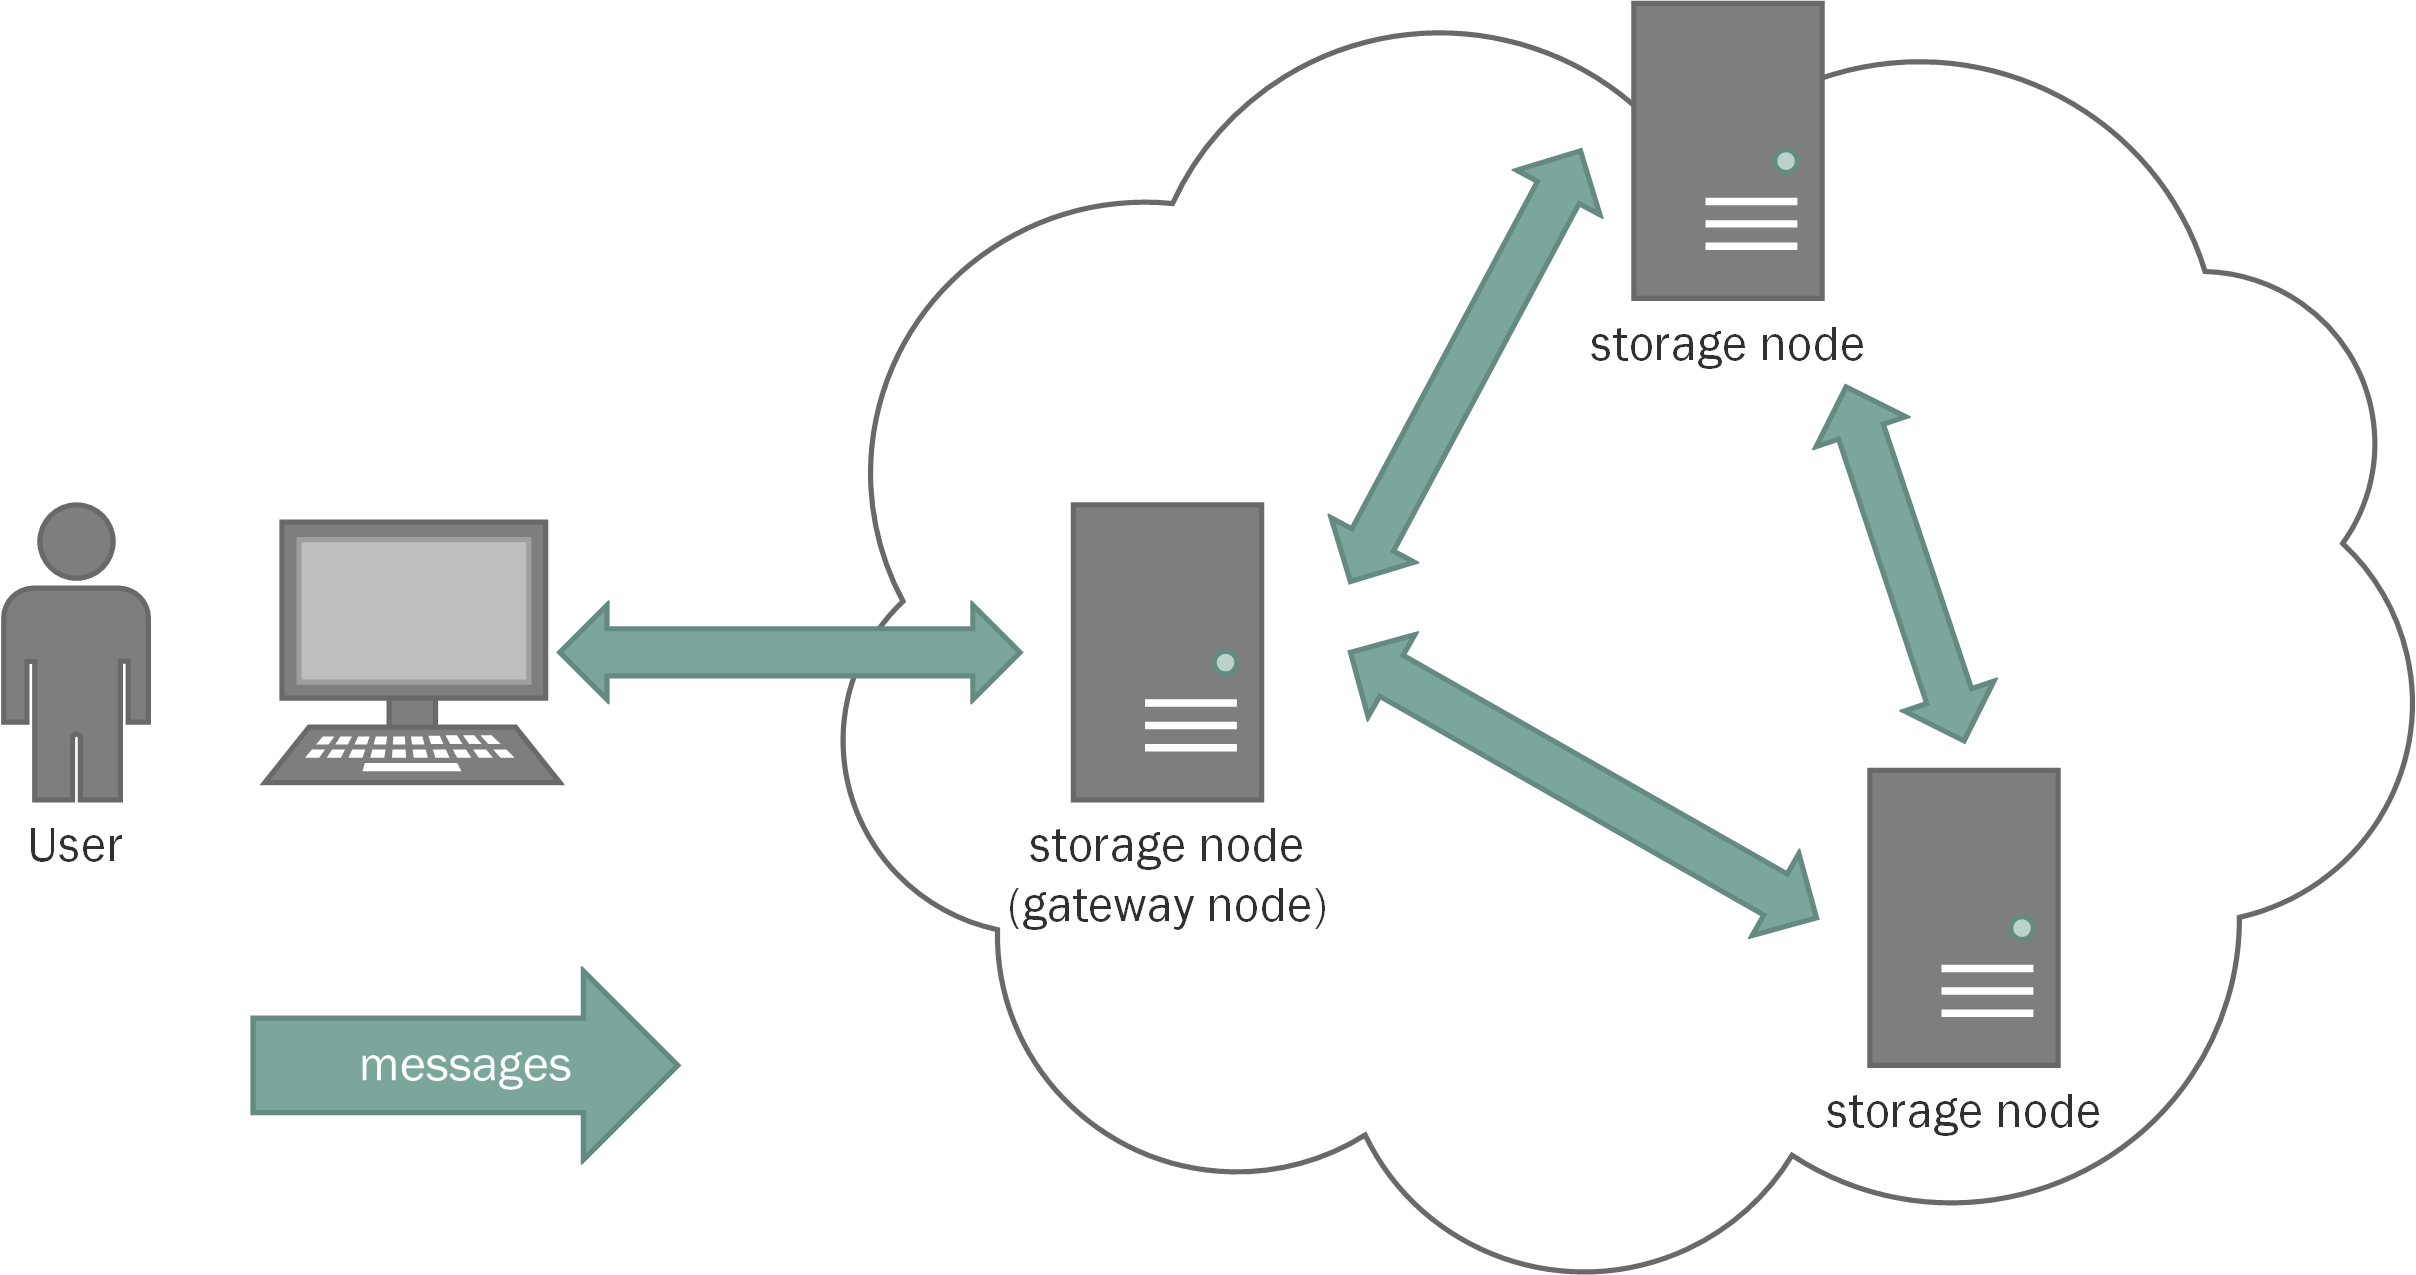
\includegraphics[width=0.8\textwidth]{arch-overview}
	\caption[Diagram architektury systemu.]{System to zdecentralizowana sieć komunikujących się ze sobą węzłów. Komunikaty, w zależności od typu, są rozgłaszane po całym systemie lub kierowane bezpośrednio do odpowiedniego węzła.}
	\label{fig:arch-overview}
\end{figure}

Użytkownik może wykonywać swoje zapytania na dowolnym z węzłów. Zawsze jednak otrzyma dostęp do wszystkich swoich plików, jakie przechowuje w systemie. Wybór węzła dostępowego (gateway node) nie powinien mieć wpływu na wydajność. W związku z tym, że każdy plik może być przechowywany w innym węźle, procedura obsługi zapytań pomija sprawdzanie czy poszukiwany plik znajduje się w aktualnym węźle dostępowym.







\subsection{Struktury}
Spośród wszystkich wymienianych między procesami i węzłami wiadomości, dla trzech z nich zostały zdefiniowane właściwe struktury (rekordy w języku Erlang). Są to struktura użytkownika (User), metadanych pliku (File), zapytania (Request), oraz akcji użytkownika (Action). Pozostałe wiadomości są zwykłymi krotkami zbudowanymi z typów prymitywnych oraz trzech poniżej przedstawianych struktur.

Są to również jedyne obiekty persystowane w bazie danych przy pomocy odpowiednich DAO.

Definicje rekordów znajdują się w pliku storage/include/shared.hrl.

\subsubsection{User}
Definicja rekordu:
\begin{lstlisting}
-record(user, {
	name 		:: nonempty_string(), 
	secret 		:: nonempty_string(), 
	create_time :: integer(), 
}).
\end{lstlisting}

Struktura User reprezentuje użytkownika końcowego systemu. Pola:
\begin{itemize}
	\item name – unikalna nazwa użytkownika / login
	\item secret – prywatny klucz użytkownika używany przy autentykacji
	\item create\_time – data (timestamp) utworzenia konta użytkownika
\end{itemize}

\subsubsection{File}
Definicja rekordu:
\begin{lstlisting}
-record(file, {
	owner 		:: nonempty_string(), 
	vpath 		:: nonempty_string(), 
	bytes 		:: integer(), 
	access_mode :: integer(), 
	create_time :: integer() 
}).
\end{lstlisting}

Struktura File gromadzi metadane dotyczące pliku w systemie. Pola:
\begin{itemize}
	\item owner – identyfikator użytkownika, właściciela pliku
	\item vpath – ścieżka do pliku (UNIX-style). Razem z owner tworzą klucz \item główny listy plików
	\item bytes – rozmiar pliku (w bajtach)
	\item access\_mode – flagi dostępu do pliku
	\item create\_time – data (timestamp) utworzenia pliku
\end{itemize}

\subsubsection{Request}
Definicja rekordu:
\begin{lstlisting}
-record(request, {
	type 				:: 'create' | 'read' | 'update'
						 | 'delete' | 'list' | 'find',
	user 				:: nonempty_string(),
	addr = {none, none} :: { nonempty_string(),
							 nonempty_string() },
	hmac = none 		:: string(), 
	data = none 		:: binary(), 
	opts = none 		:: term() 
}).
\end{lstlisting}

Struktura Request reprezentuje żądanie operacji na pliku. Jest to również podstawowy typ wiadomości w systemie. Przekazywane jest zarówno pomiędzy węzłami jak i wewnątrz węzłów między poszczególnymi modułami. Pola:
\begin{itemize}
	\item type – atom reprezentujący jeden z typów operacji
	\item user – identyfikator użytkownika wykonującego zapytanie
	\item addr - krotka reprezentująca adres żądanego pliku, w postaci \{owner, vpath\}
	\item hmac – suma kontrolna HMAC (więcej w rozdziale dotyczącym autentykacji)
	\item data – binarne dane (w przypadku tworzenia / aktualizacji pliku)
	\item opts – obecnie nie używane
\end{itemize}

\subsubsection{Action}
Definicja rekordu:
\begin{lstlisting}
-record(action, {
	user_id 		:: nonempty_string(), 
	file_id 		, 
	weight 			:: integer(), 
	action_time 	:: integer(), 
	action_type 	:: nonempty_string() 
}).
\end{lstlisting}

Struktura Action tworzona jest przy przetwarzaniu zapytania Request a następnie zapisywana w bazie danych. Lista takich struktur daje opis historii operacji danego użytkownika. Pola:
\begin{itemize}
	\item user\_id – identyfikator użytkownika
	\item file\_id – adres pliku
	\item weight – waga przypisana żądaniu podczas schedulingu
	\item action\_time – data (timestamp) obsługi żądania
	\item action\_type – identycznie jak request\#type, tylko w postaci string()
\end{itemize}





\subsection{Storage}
Pojedynczy węzeł systemu jest aplikacją Erlang/OTP. Składa się z jednego, głównego supervisora zarządzającego pięcioma gen\_serverami: storage\_http\_srv, storage\_auth\_srv, storage\_dist\_srv, storage\_core\_srv oraz storage\_uuid\_srv. storage\_http\_srv jest opcjonalny a jego obecność nie jest wymagana do poprawnej pracy całego systemu. Supervisor pracuje w polityce one-for-one, restartując poszczególne komponenty w razie awarii. Struktura serwerów przedstawiona jest na \autoref{fig:supervision}.

Każdy z gen\_serverów ma jasno określone zadania. Poszczególne serwery (moduły) ściśle współpracują między sobą i wymieniają wiadomości w celu obsługi zapytania. Na podstawie przepływu informacji między nimi można wyróżnić warstwową hierarchię przedstawioną na \autoref{fig:node-overview}. Zapytanie przekazywane jest między kolejnymi modułami:
\begin{enumerate}
	\item storage\_http\_srv (opcjonalnie)
	\item storage\_auth\_srv
	\item storage\_dist\_srv
	\item storage\_core\_srv
\end{enumerate}

Użycie modułu storage\_http\_srv jest opcjonalne – użytkownik może również skorzystać z biblioteki klienckiej (napisanej w Erlangu) i pominąć wysyłanie zapytania przez protokół HTTP.

Szczegółowy opis kolejnych faz obsługi zapytania znajduje się w podrozdziale dotyczącym komunikacji wysokopoziomowej.

\begin{figure}[!htbp]
	\centering
	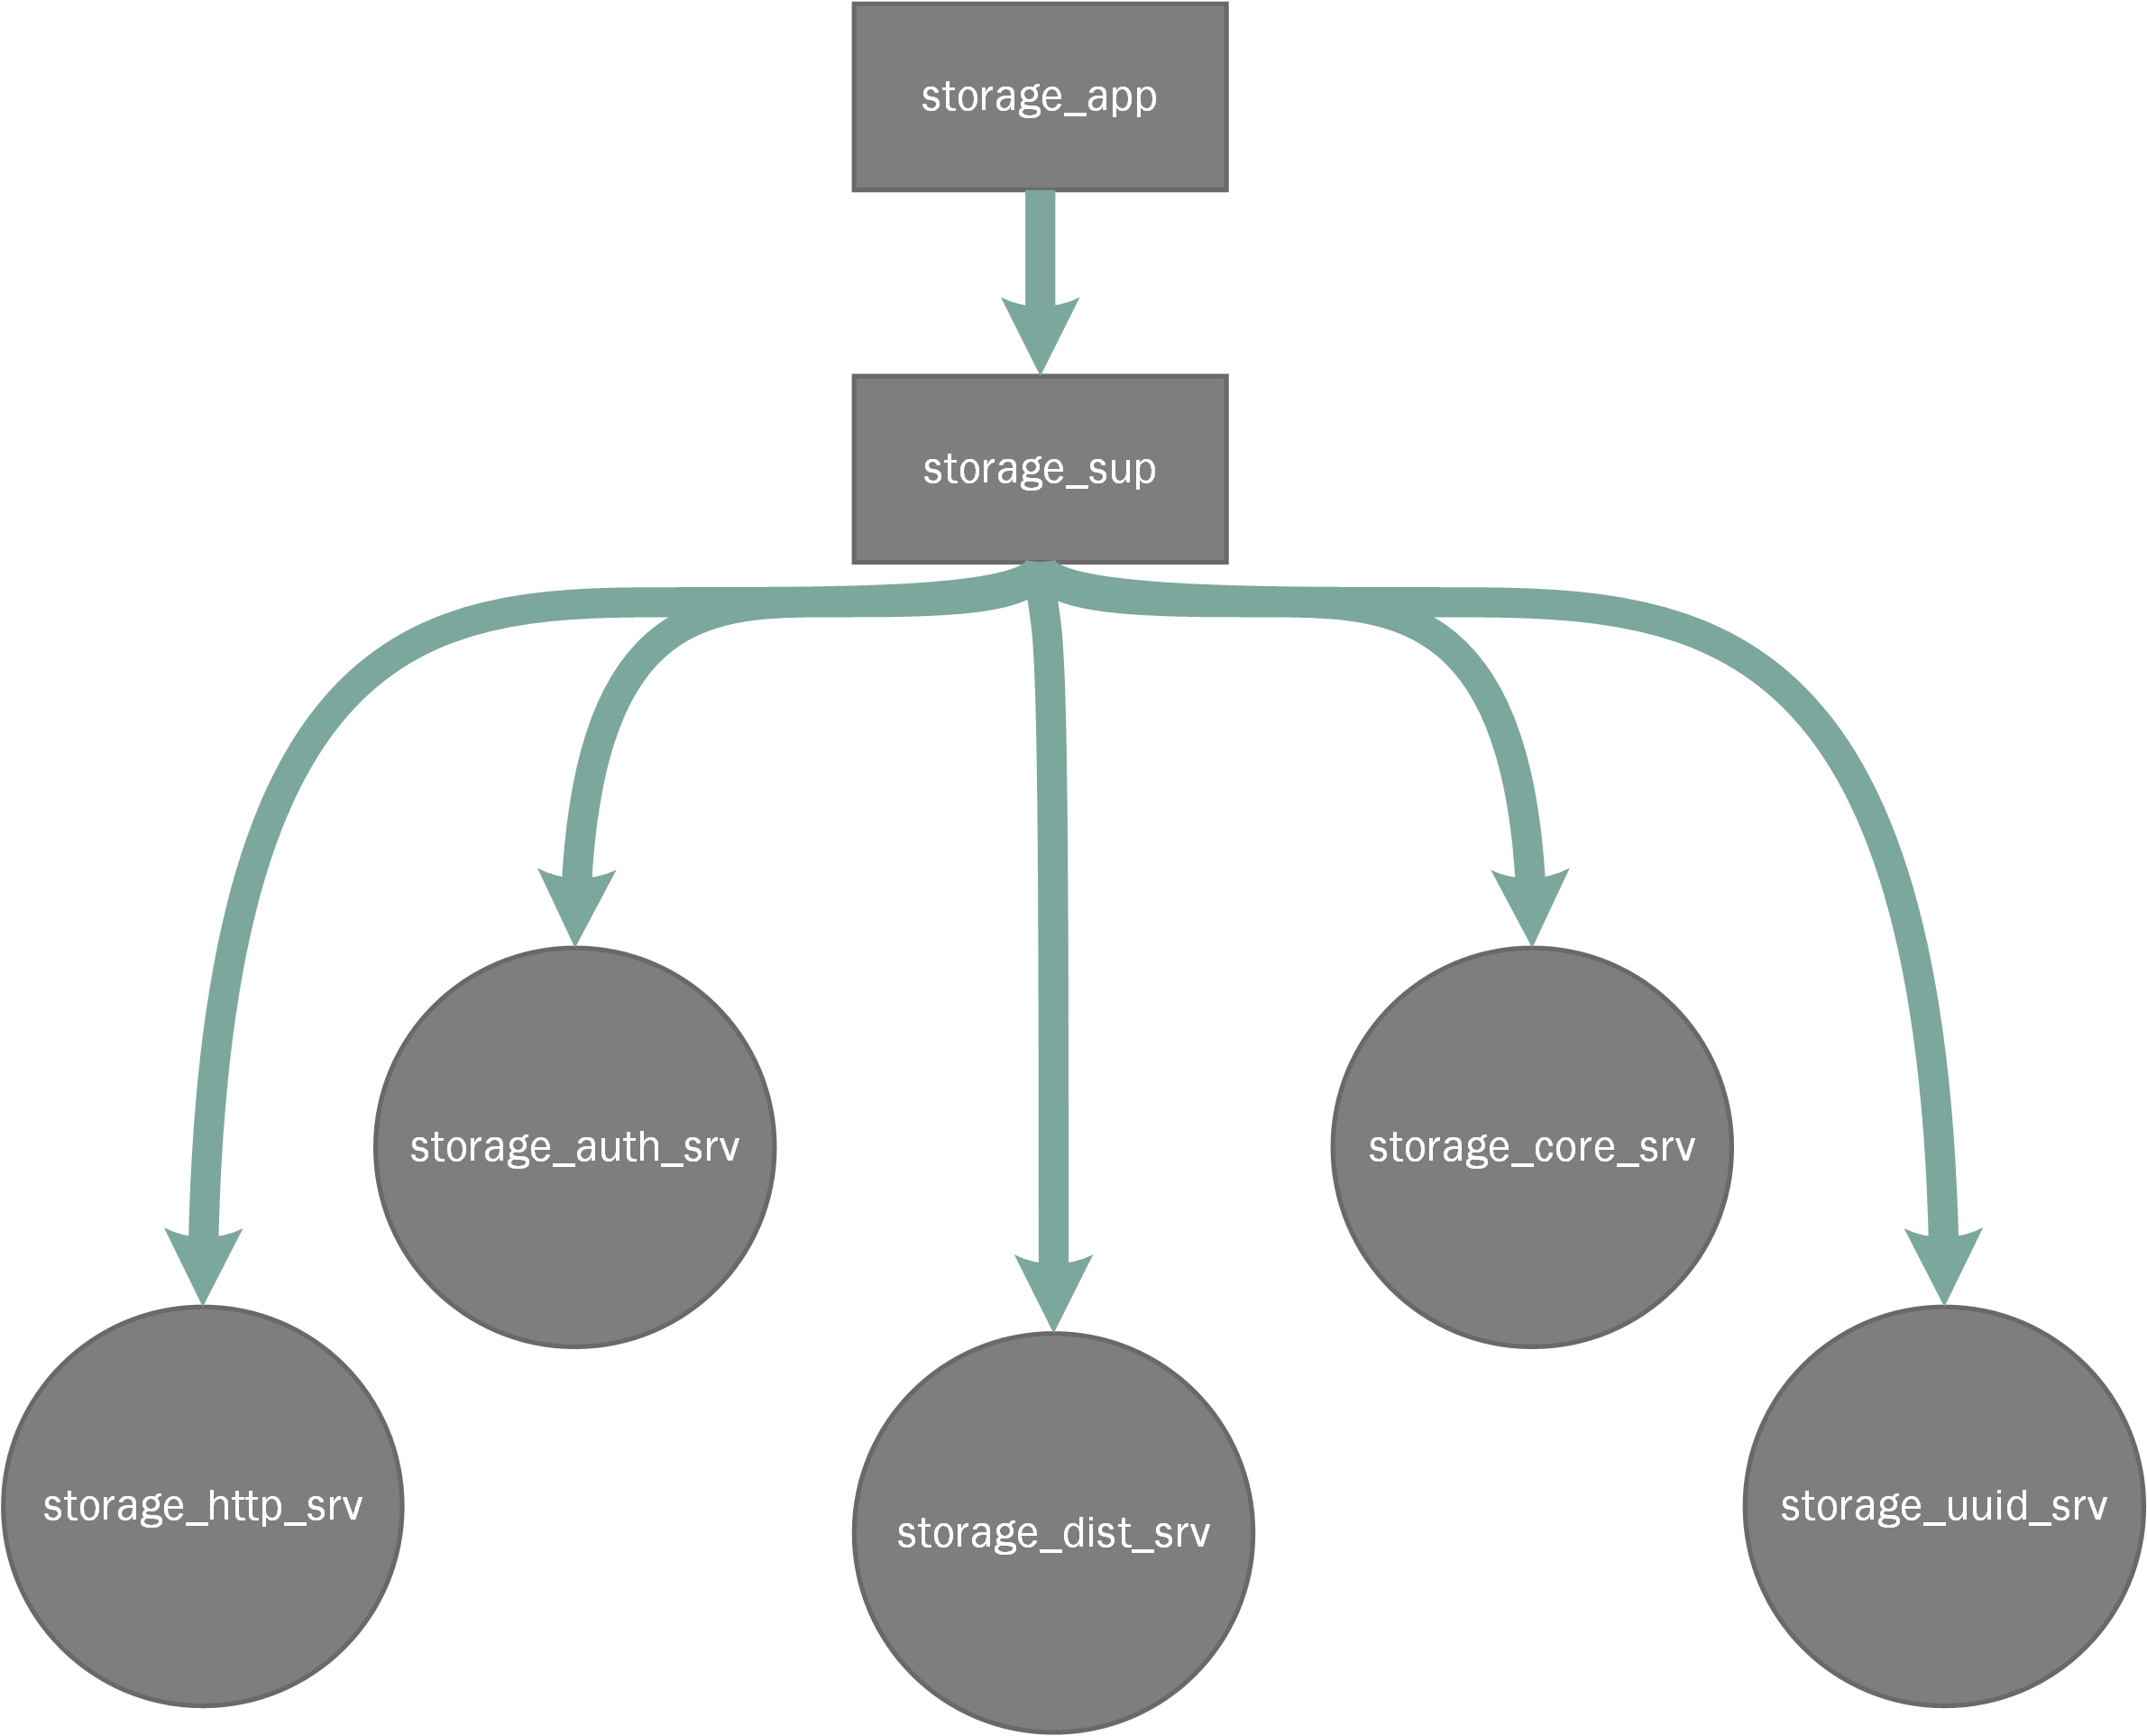
\includegraphics[width=0.8\textwidth]{supervision}
	\caption[Supervision tree.]{Supervision tree. Aplikacja zbudowana jest z pięciu gen\_serverów. Każdy jest osobnym procesem. Ponadto storage\_core\_srv zarządza pulą procesów wykonawczych.}
	\label{fig:supervision}
\end{figure}

\begin{figure}[!htbp]
	\centering
	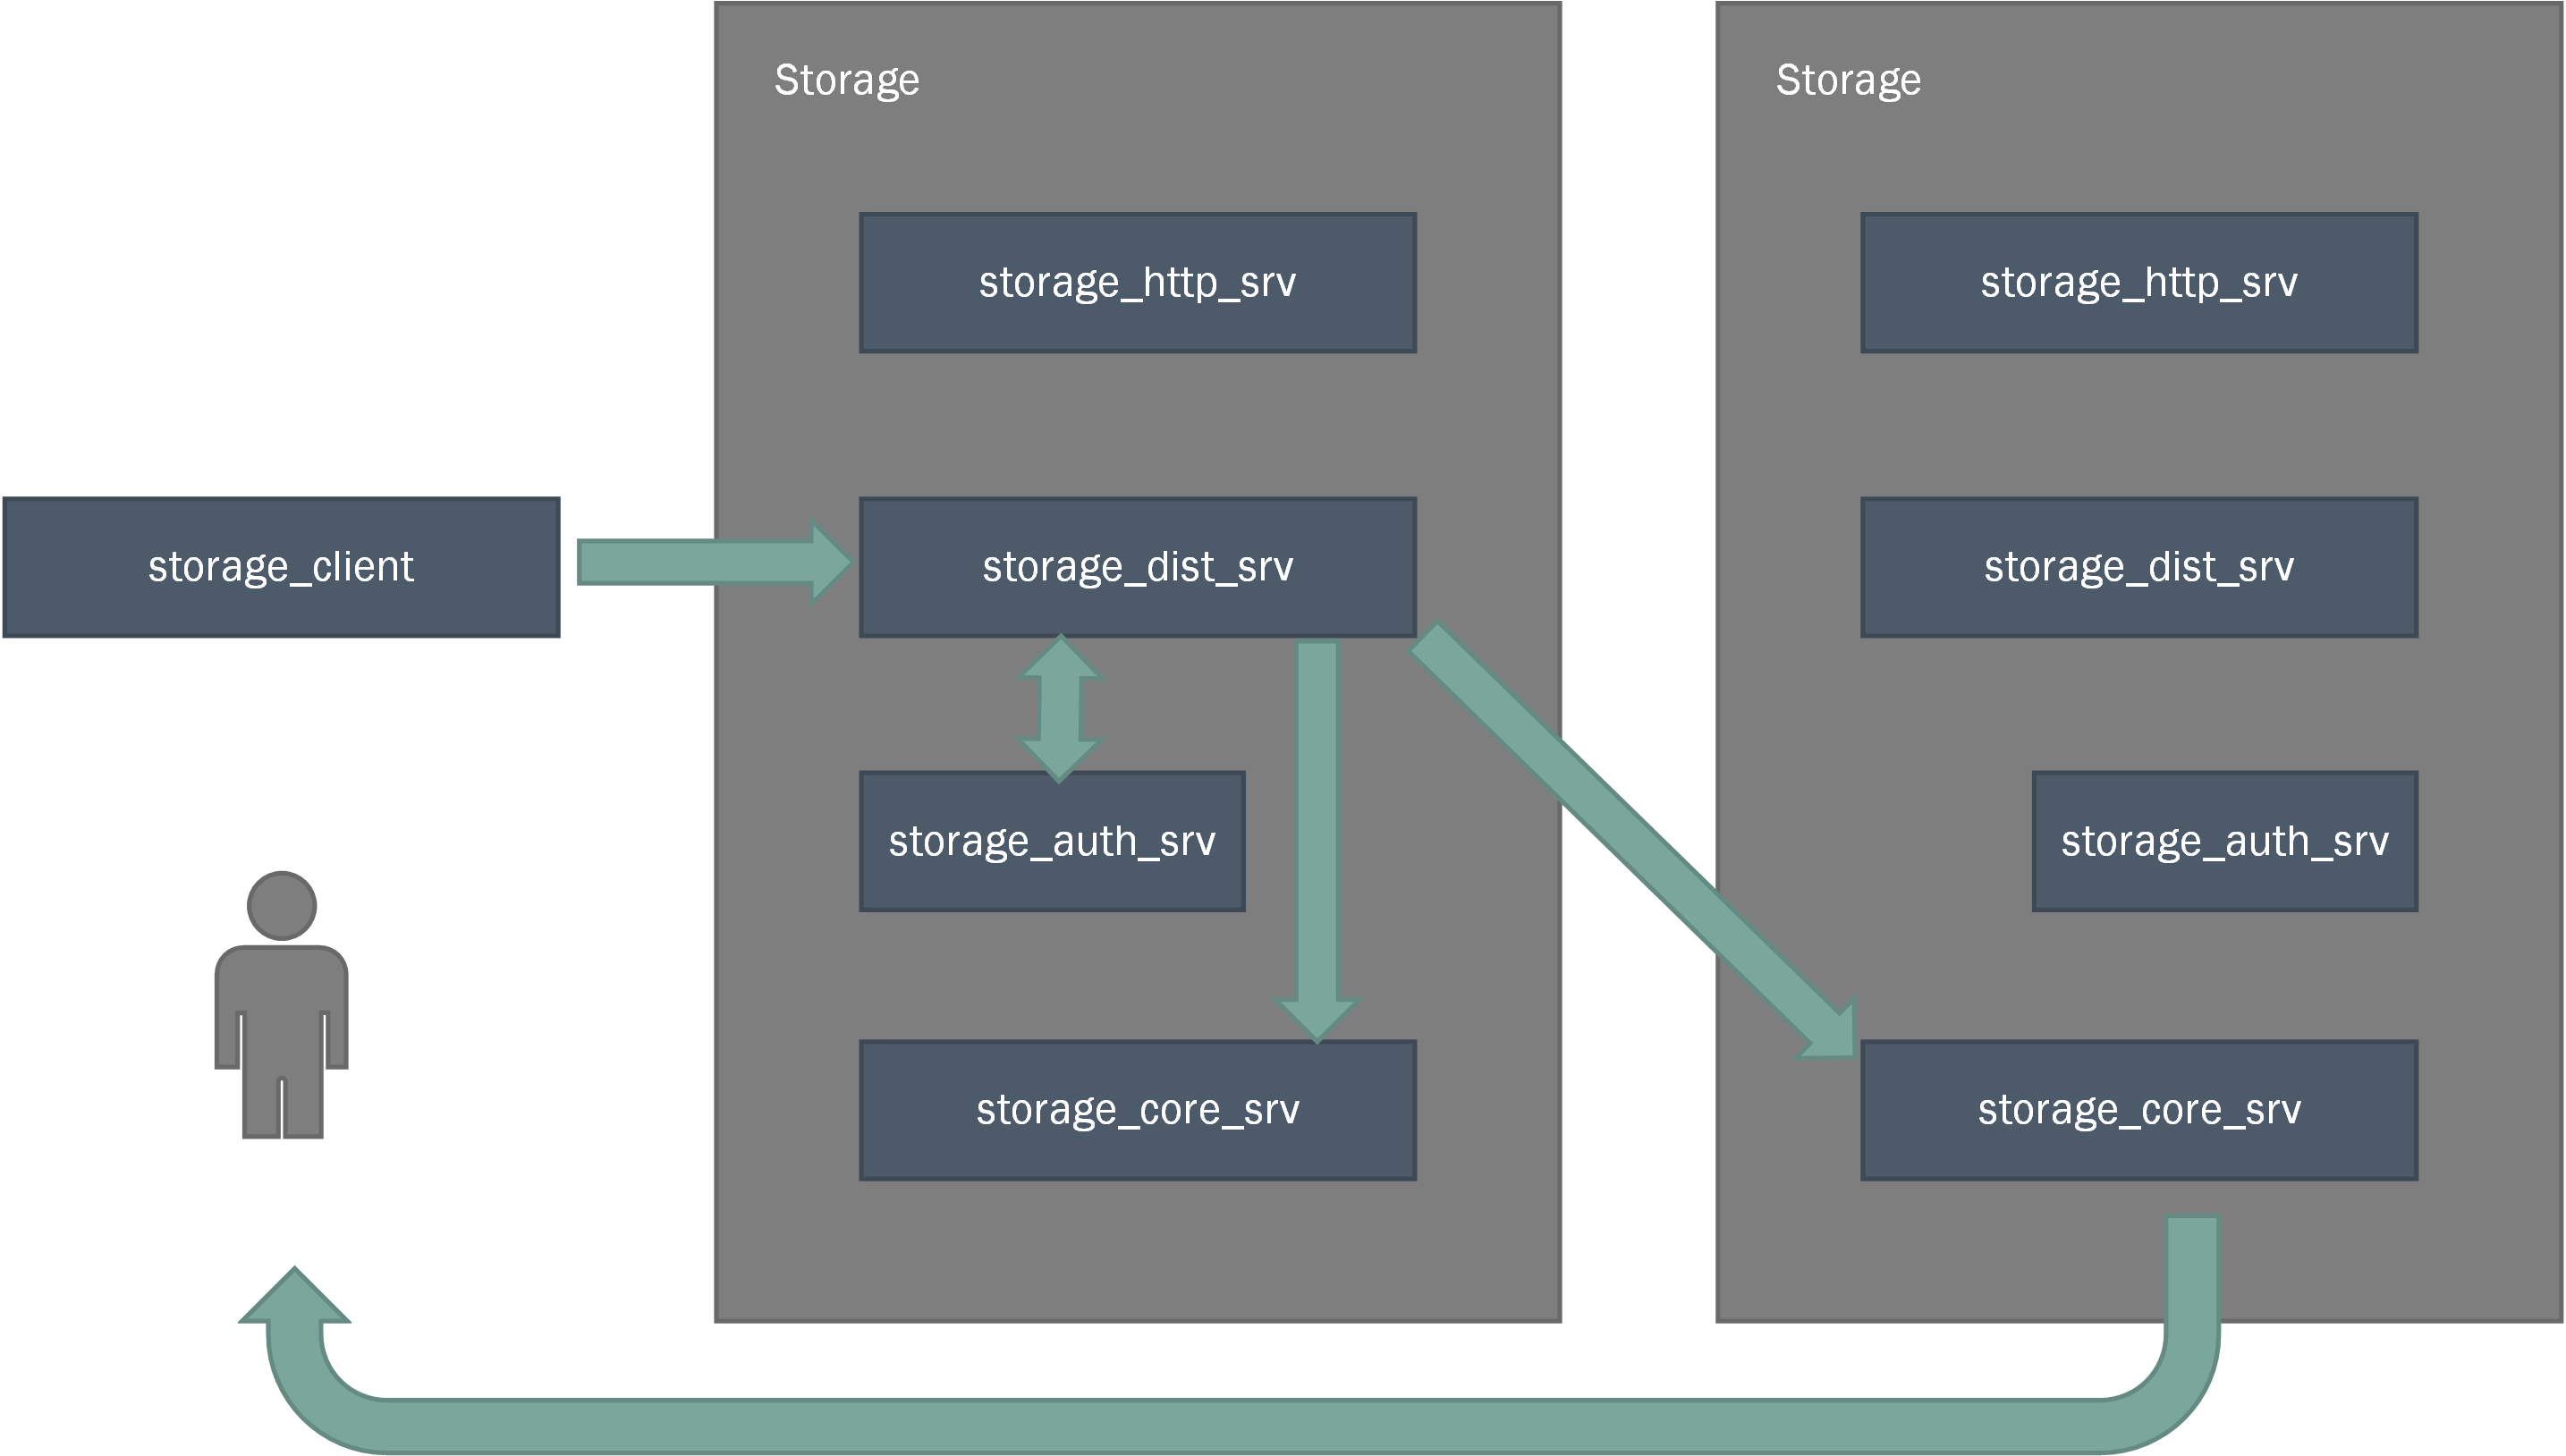
\includegraphics[width=0.8\textwidth]{node-overview}
	\caption[Przepływ zapytania w systemie.]{Przepływ zapytania w systemie. Zapytanie jest rozgłaszane do wszystkich węzłów. Zielone linie oznaczają przepływ zapytania.}
	\label{fig:node-overview}
\end{figure}

\subsubsection{Komunikacja wysokopoziomowa}
Komunikacja pomiędzy węzłami oparta jest w całości na przesyłaniu struktur Request. W zależności od typu zapytania, w procedurze obsługi występują nieznaczne różnice. Można jednak przedstawić to w postaci listy modułów, gdzie kolejno trafia zapytanie:

\begin{enumerate}
	\item (opcjonalnie) storage\_http\_srv – zapytanie jest parsowane, tworzona jest struktura Request
	\item storage\_dist\_srv – przyjmuje strukturę Request, przekazuje do autentykacji
	\item storage\_auth\_srv – autentykuje i sprawdza spójność przekazanego zapytania
	\item storage\_dist\_srv
	\begin{enumerate}
		\item zapytania create / update – wyszukuje odpowiedni węzeł i przekazuje strukturę Request do działającego na nim storage\_core\_srv
		\item pozostałe zapytania – rozgłasza strukturę Request do serwerów storge\_core\_srv na wszystkich węzłach w systemie
	\end{enumerate}
	\item storage\_core\_srv – dokonuje obsługi zapytania lub odrzuca je, jeżeli dotyczy pliku który nie znajduje się w danym węźle. Odpowiedź kierowana jest prosto do użytkownika
\end{enumerate}

\begin{figure}[!htbp]
	\centering
	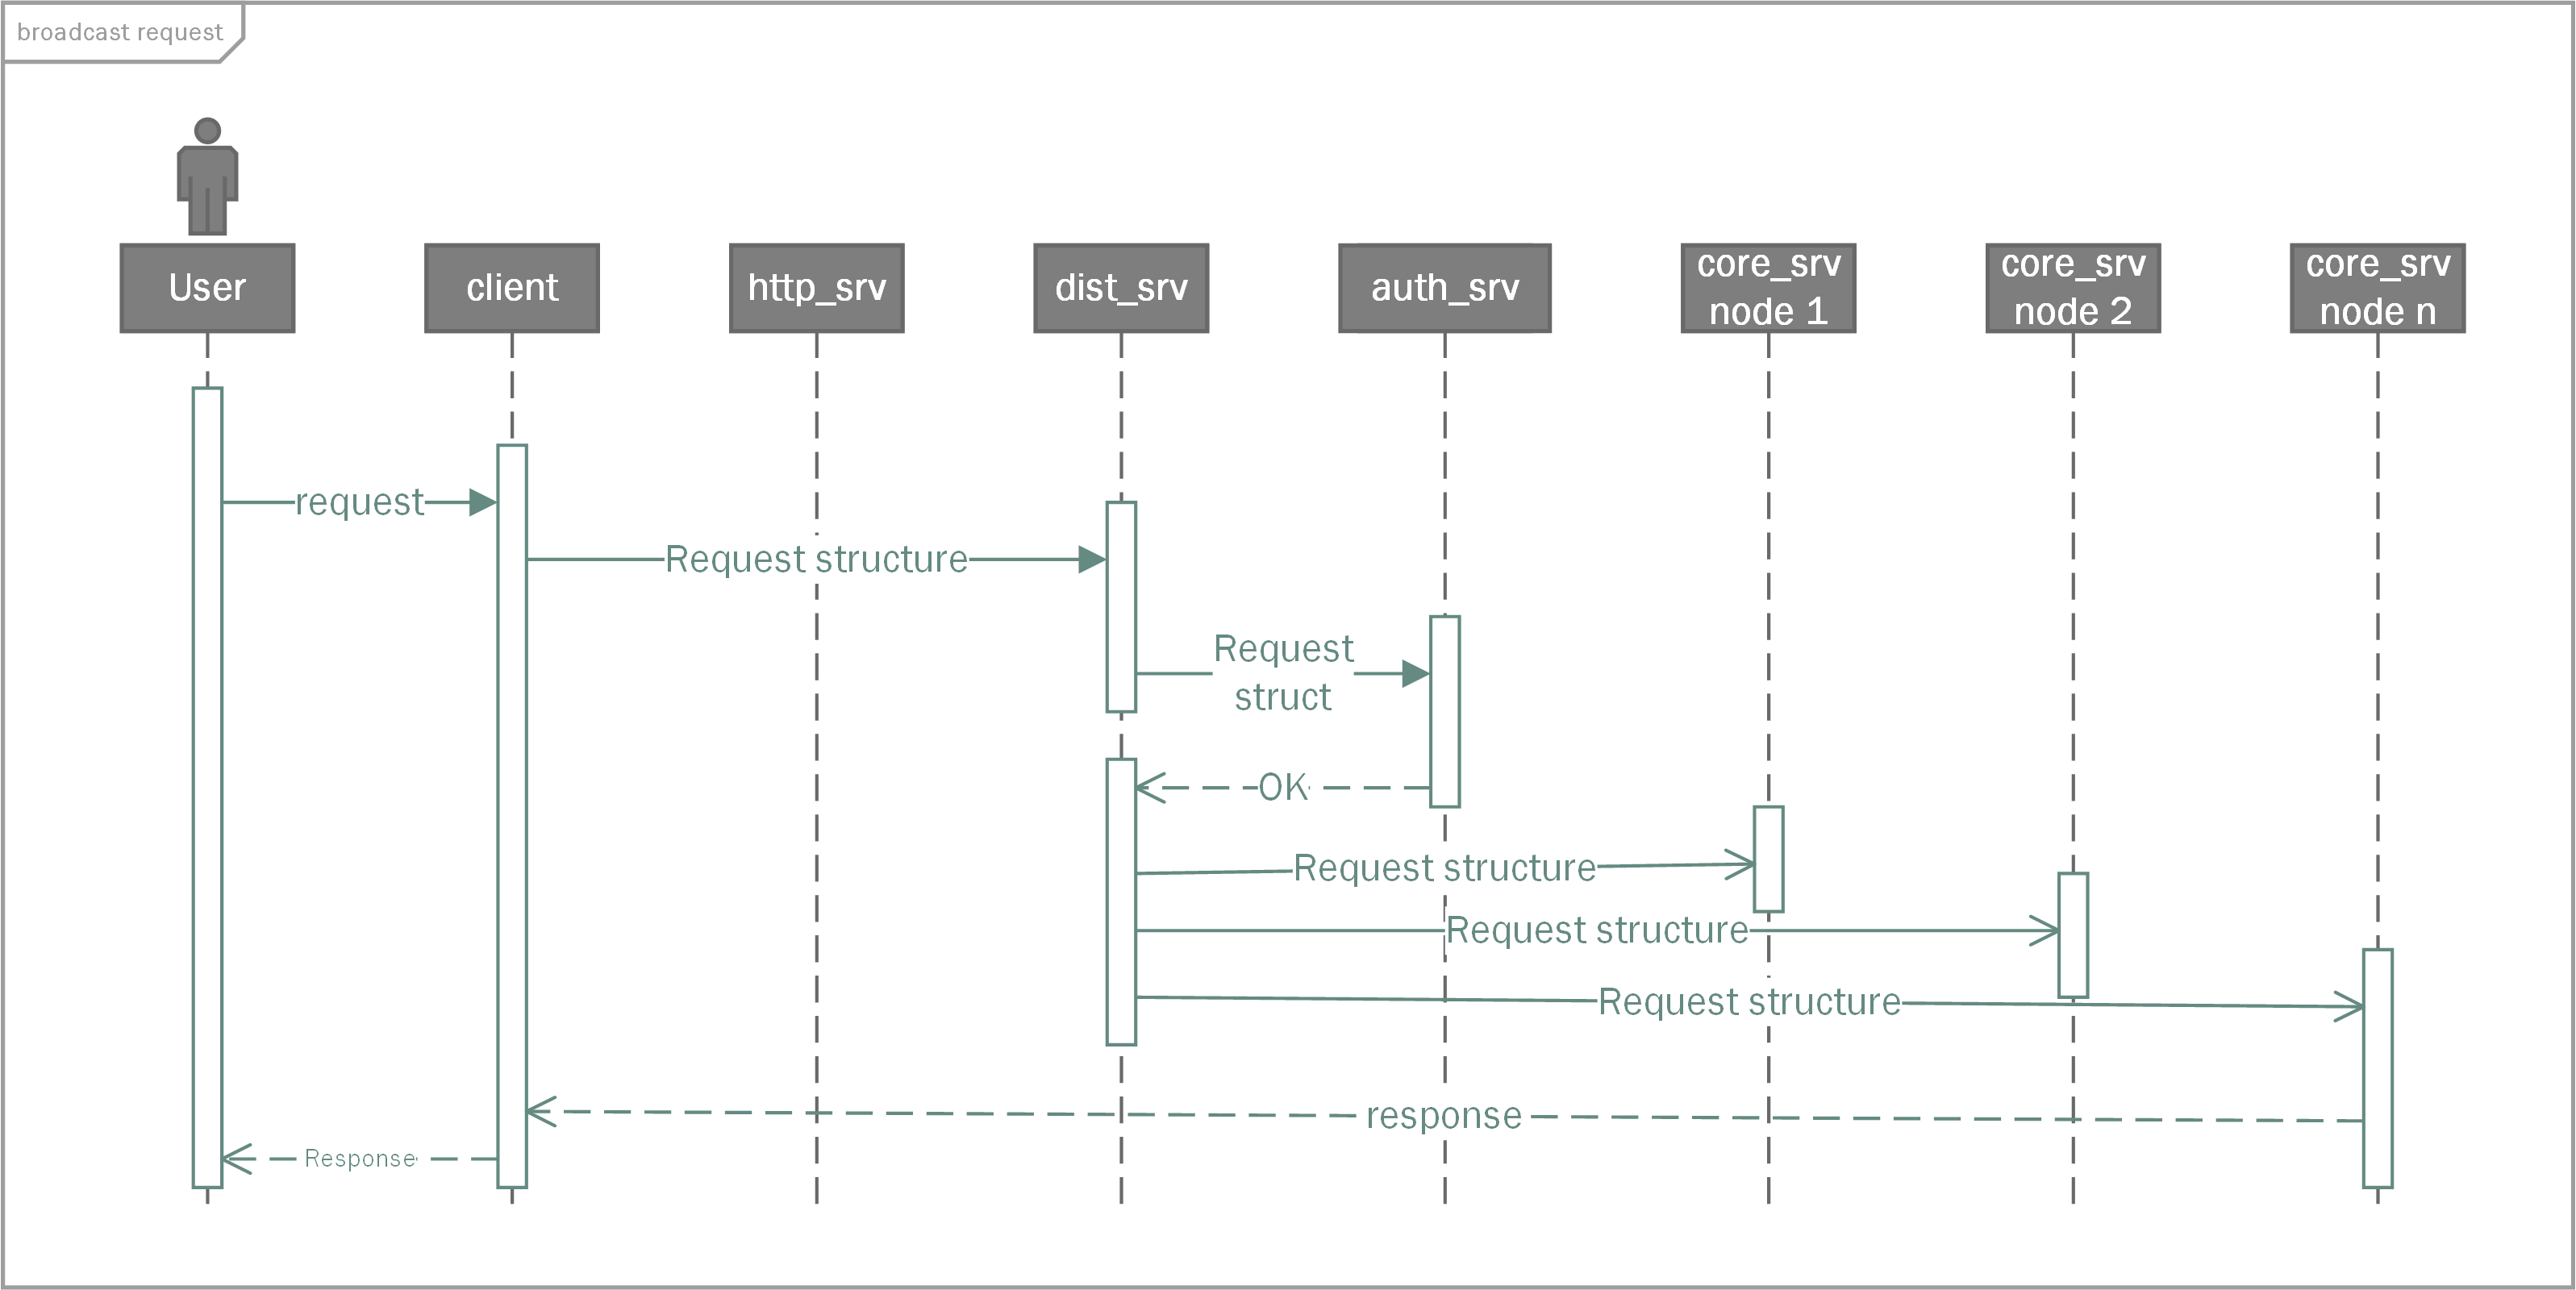
\includegraphics[width=0.9\textwidth]{broadcast-seq}
	\caption[Zapytanie rozgłoszeniowe (Erlang).]{Zapytanie rozgłoszeniowe z wykorzystaniem biblioteki klienckiej zakończone powodzeniem.}
	\label{fig:broadcast-seq}
\end{figure}

\autoref{fig:broadcast-seq} pokazuje diagram sekwencji obsługi zapytań rozgłoszeniowych z wykorzystaniem biblioteki klienckiej. Zapytania tego typu to zapytania read, delete oraz find. \autoref{fig:broadcast-http-seq} pokazuje te same akcje przy wykorzystaniu modułu HTTP. Widać, że moduł HTTP wewnętrznie korzysta z biblioteki klienckiej. Rysunki zakładają, że autentykacja przebiegła pomyślnie a jeden z węzłów zawierał żądany plik. Użytkownikowi odpowiada tylko jeden węzeł - ten, który obsłużył zapytanie (przechowywał poszukiwany plik). Pozostałe węzły ignorują komunikat.

\begin{figure}[!htbp]
	\centering
	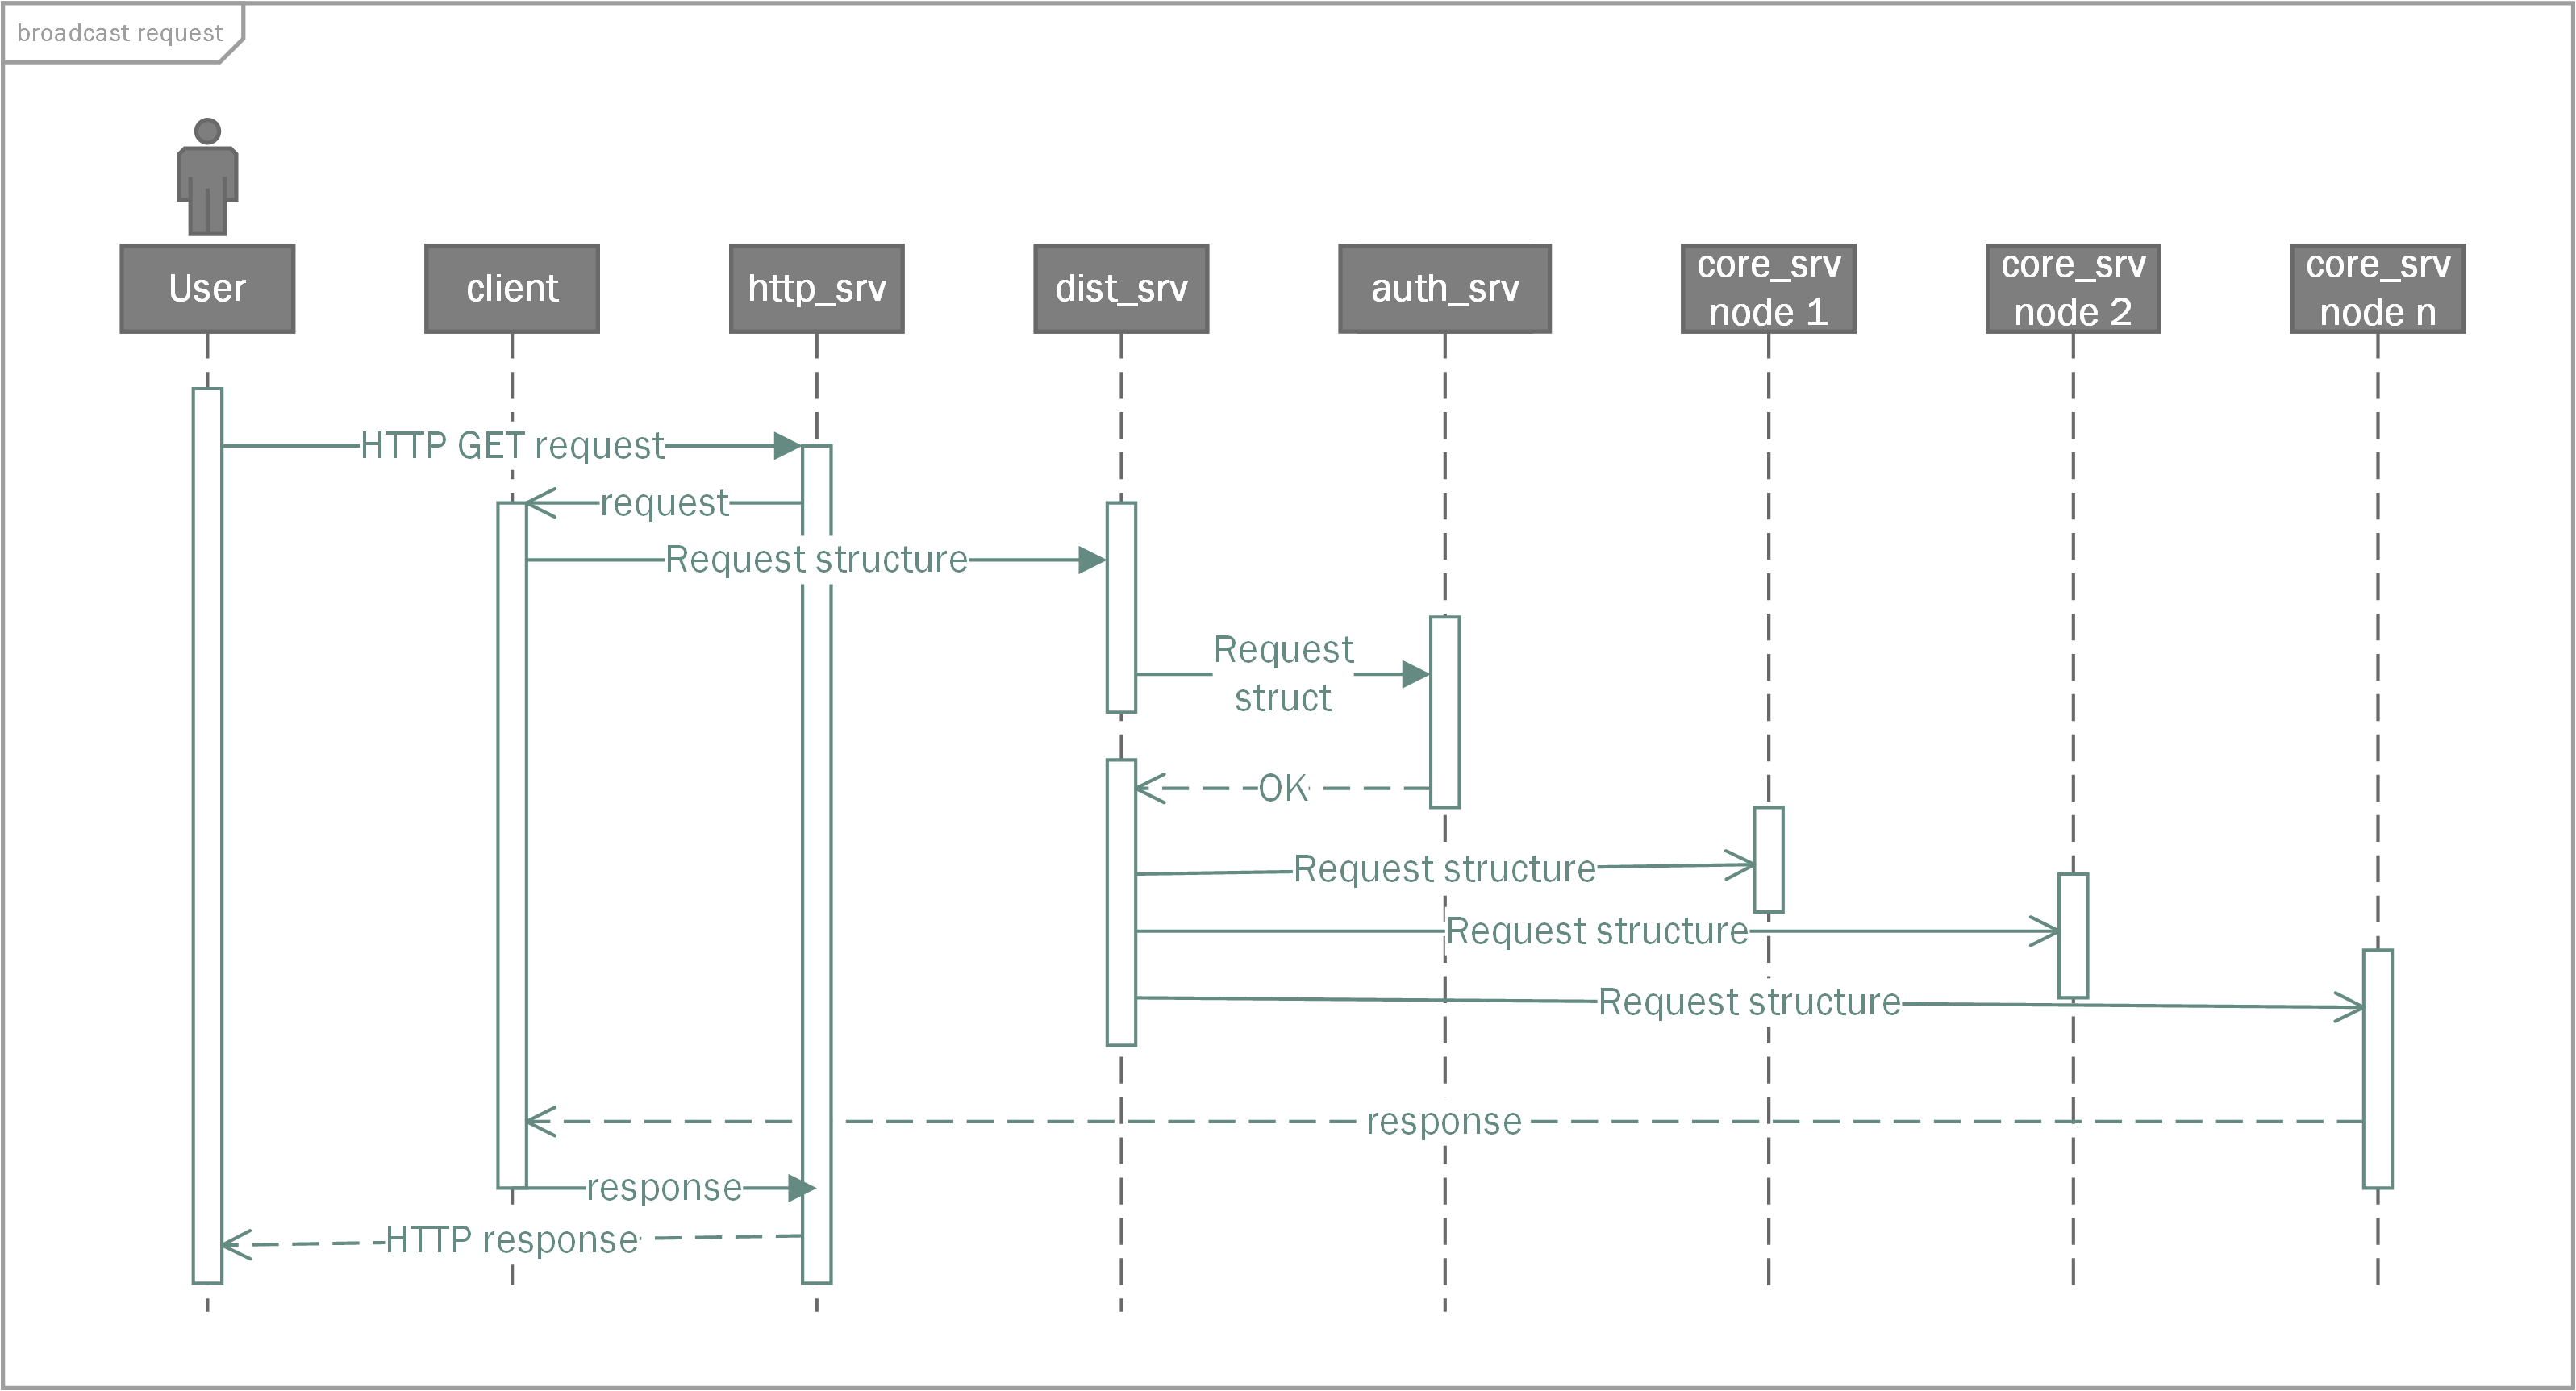
\includegraphics[width=0.9\textwidth]{broadcast-http-seq}
	\caption[Zapytanie rozgłoszeniowe (HTTP).]{Zapytanie rozgłoszeniowe z wykorzystaniem modułu HTTP. Użytkownik wysyła zapytanie metodą GET, które tłumaczone jest na odpowiednią strukturę Request.}
	\label{fig:broadcast-http-seq}
\end{figure}

Zapytania typu create i update nie są rozgłaszane. Najbardziej odpowiedni na przyjęcie nowych danych węzeł jest wybierany spośród wszystkich węzłów w systemie. Wybór ten dokonywany jest w węźle, do którego początkowo trafia zapytanie (gateway node). Jedyną różnicą w stosunku do \autoref{fig:broadcast-seq} oraz \autoref{fig:broadcast-http-seq} byłoby zaznaczenie pojedynczego modułu core\_srv, działającego na docelowym węźle.

W przypadku zapytania o listę wszystkich plików (zapytanie list), przeszukane muszą zostać wszystkie węzły. Odpowiedź nie wraca jednak z każdego z nich bezpośrednio do klienta, lecz do modułu dist\_srv, odpowiedzialnego za połączenie wszystkich list w jedną listę wynikową. Sytuację tę przedstawia diagram na \autoref{fig:broadcast-list}.

\begin{figure}[!htbp]
	\centering
	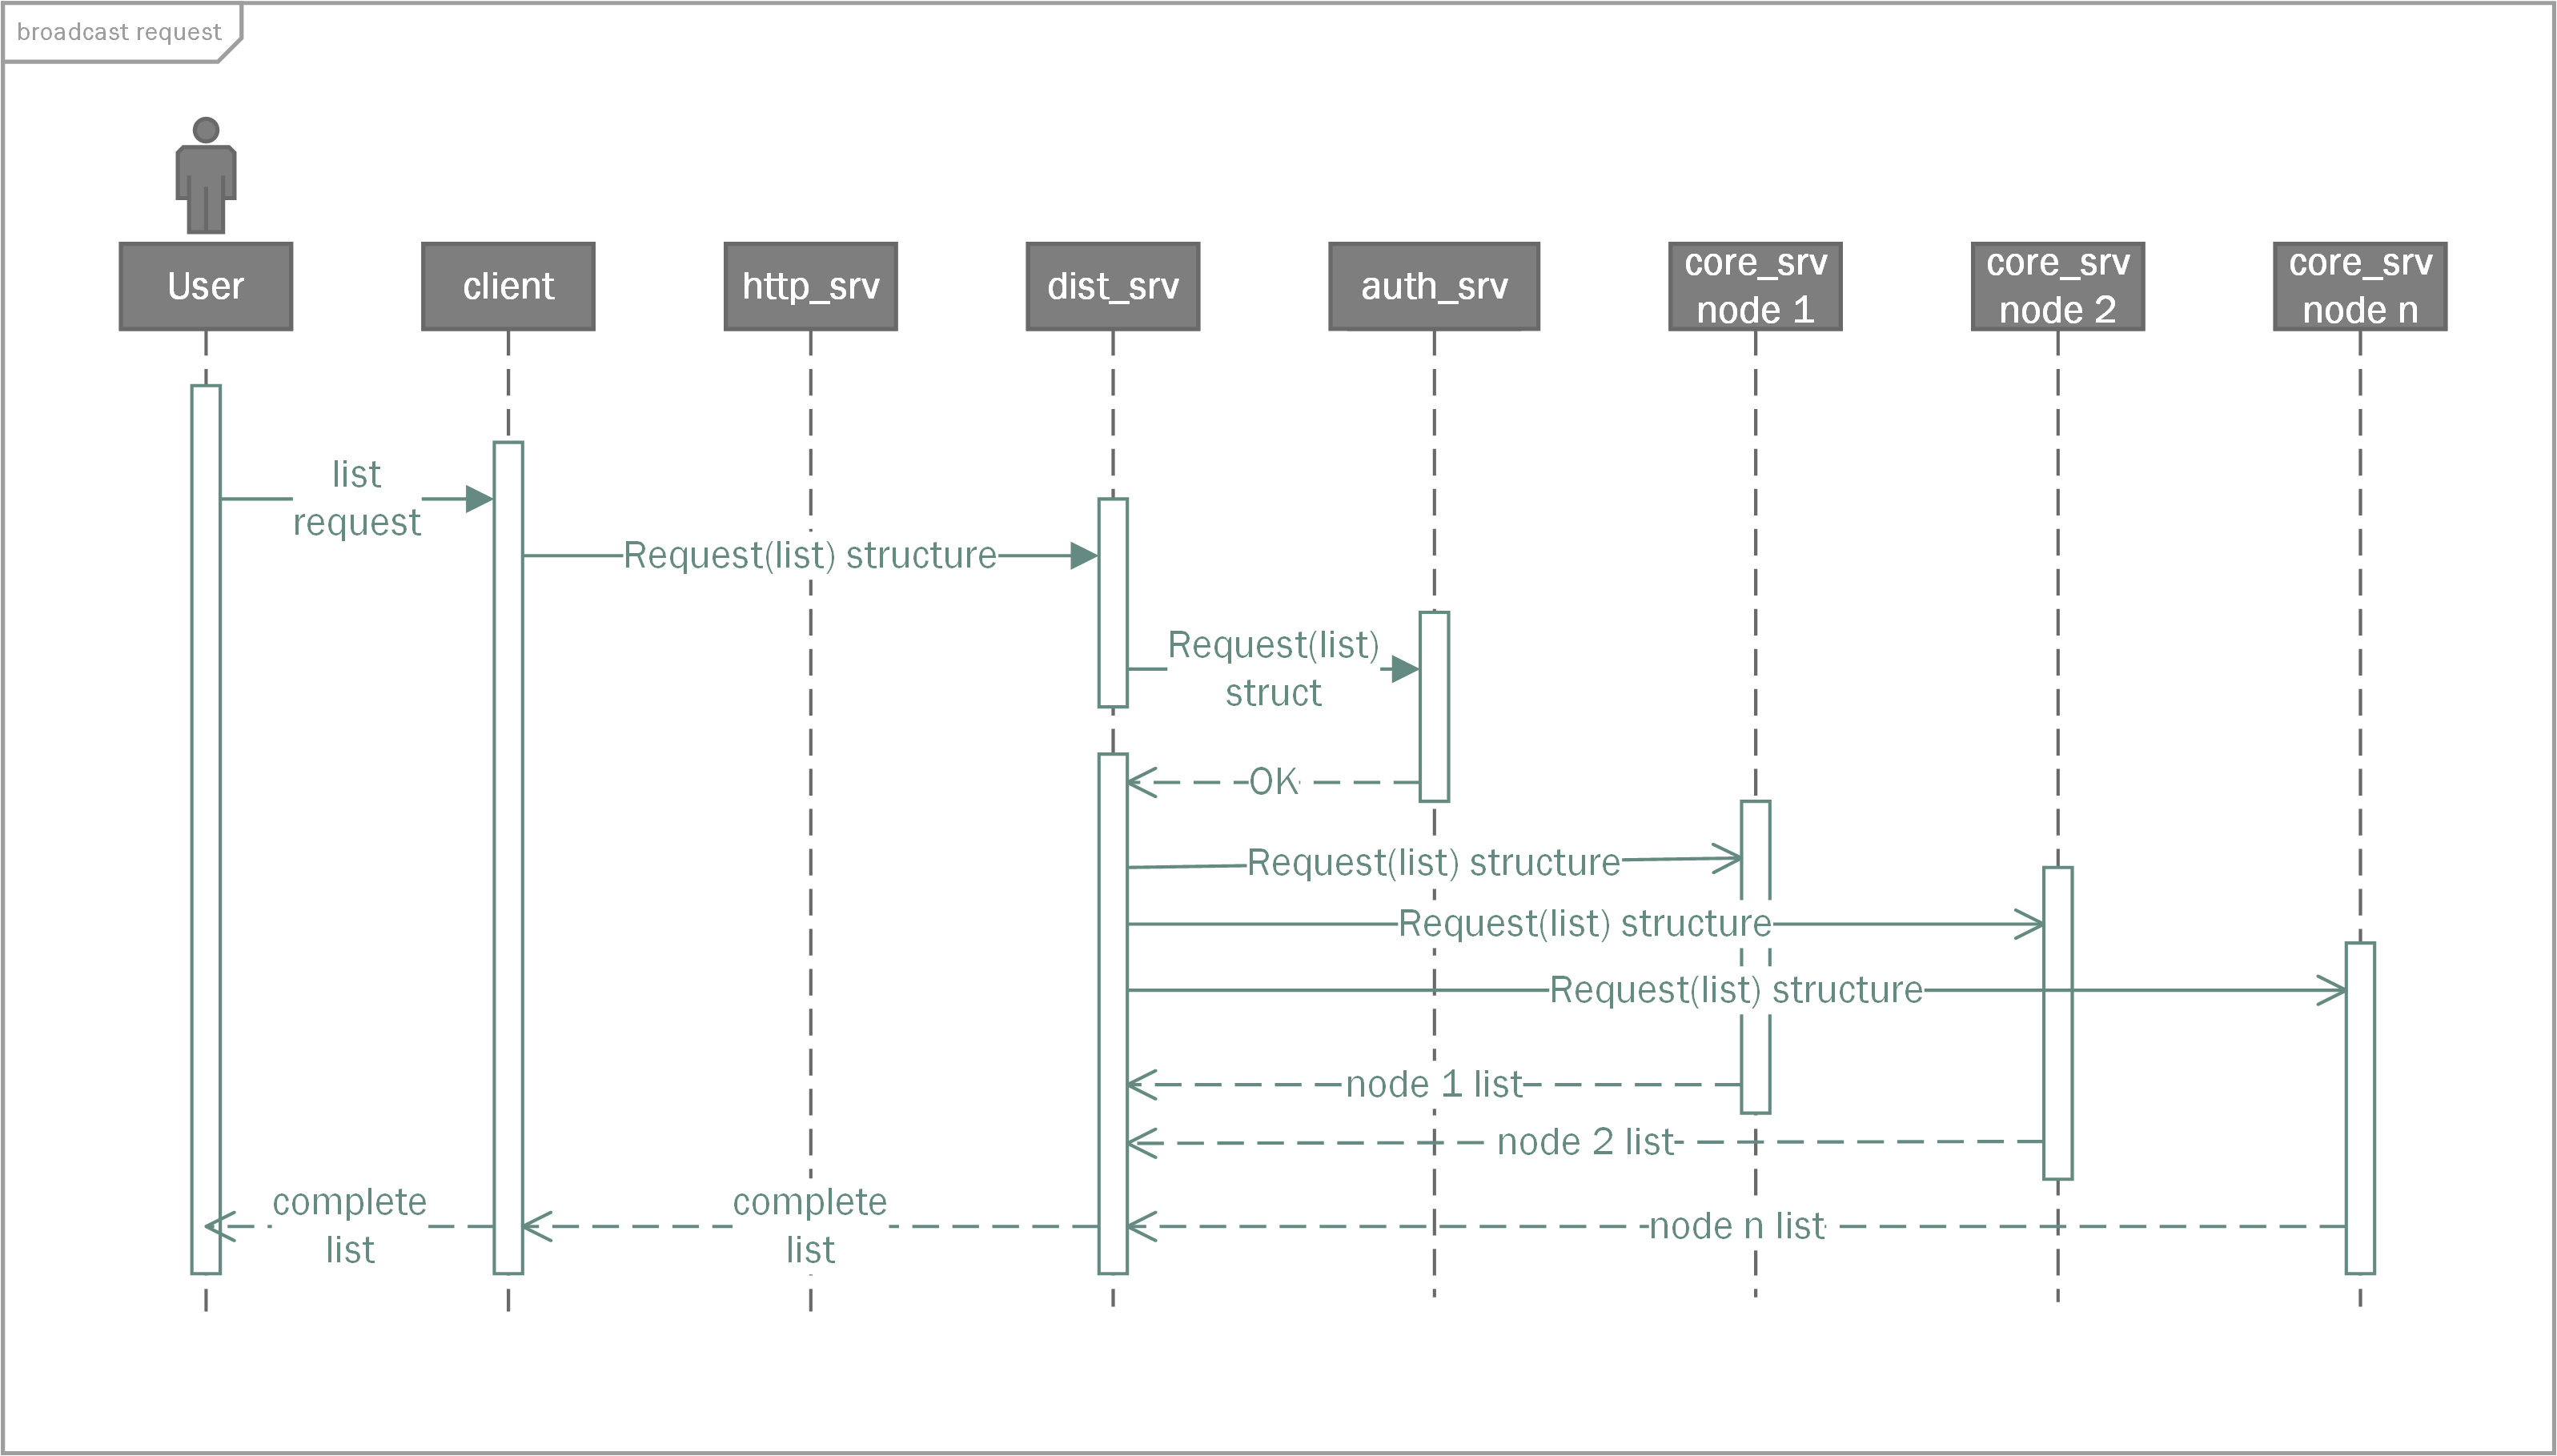
\includegraphics[width=0.9\textwidth]{broadcast-list}
	\caption[Zapytanie o listę plików.]{Obsługa zapytania o listę wszystkich plików użytkownika.}
	\label{fig:broadcast-list}
\end{figure}

\subsubsection{Obsługa błędnych zapytań}
Istnieją sytuacje, kiedy żądanie przesłane do systemu kończy się niepowodzeniem – kiedy nie udało się znaleźć pliku który użytkownik chciał odczytać lub w systemie nie ma miejsca na stworzenie nowego pliku. Można rozróżnić tutaj dwa scenariusze: system od razu sygnalizuje błąd oraz system 'zawiesza się', w oczekiwaniu na odpowiedź jednego z węzłów. 

Pierwszy ma miejsce w przypadki zapytań create i update, kiedy moduł storage\_dist\_srv zwraca do biblioteki klienckiej błąd o niemożliwości zapisania pliku. Wszystkie pozostałe zapytania (zapytania rozgłoszeniowe) mają ustalony pewien czas (domyślnie 10 sekund), po którym jeżeli biblioteka kliencka nie otrzyma odpowiedzi, zgłasza błąd. Taki scenariusz przedstawia \autoref{fig:broadcast-error}.

\begin{figure}[!htbp]
	\centering
	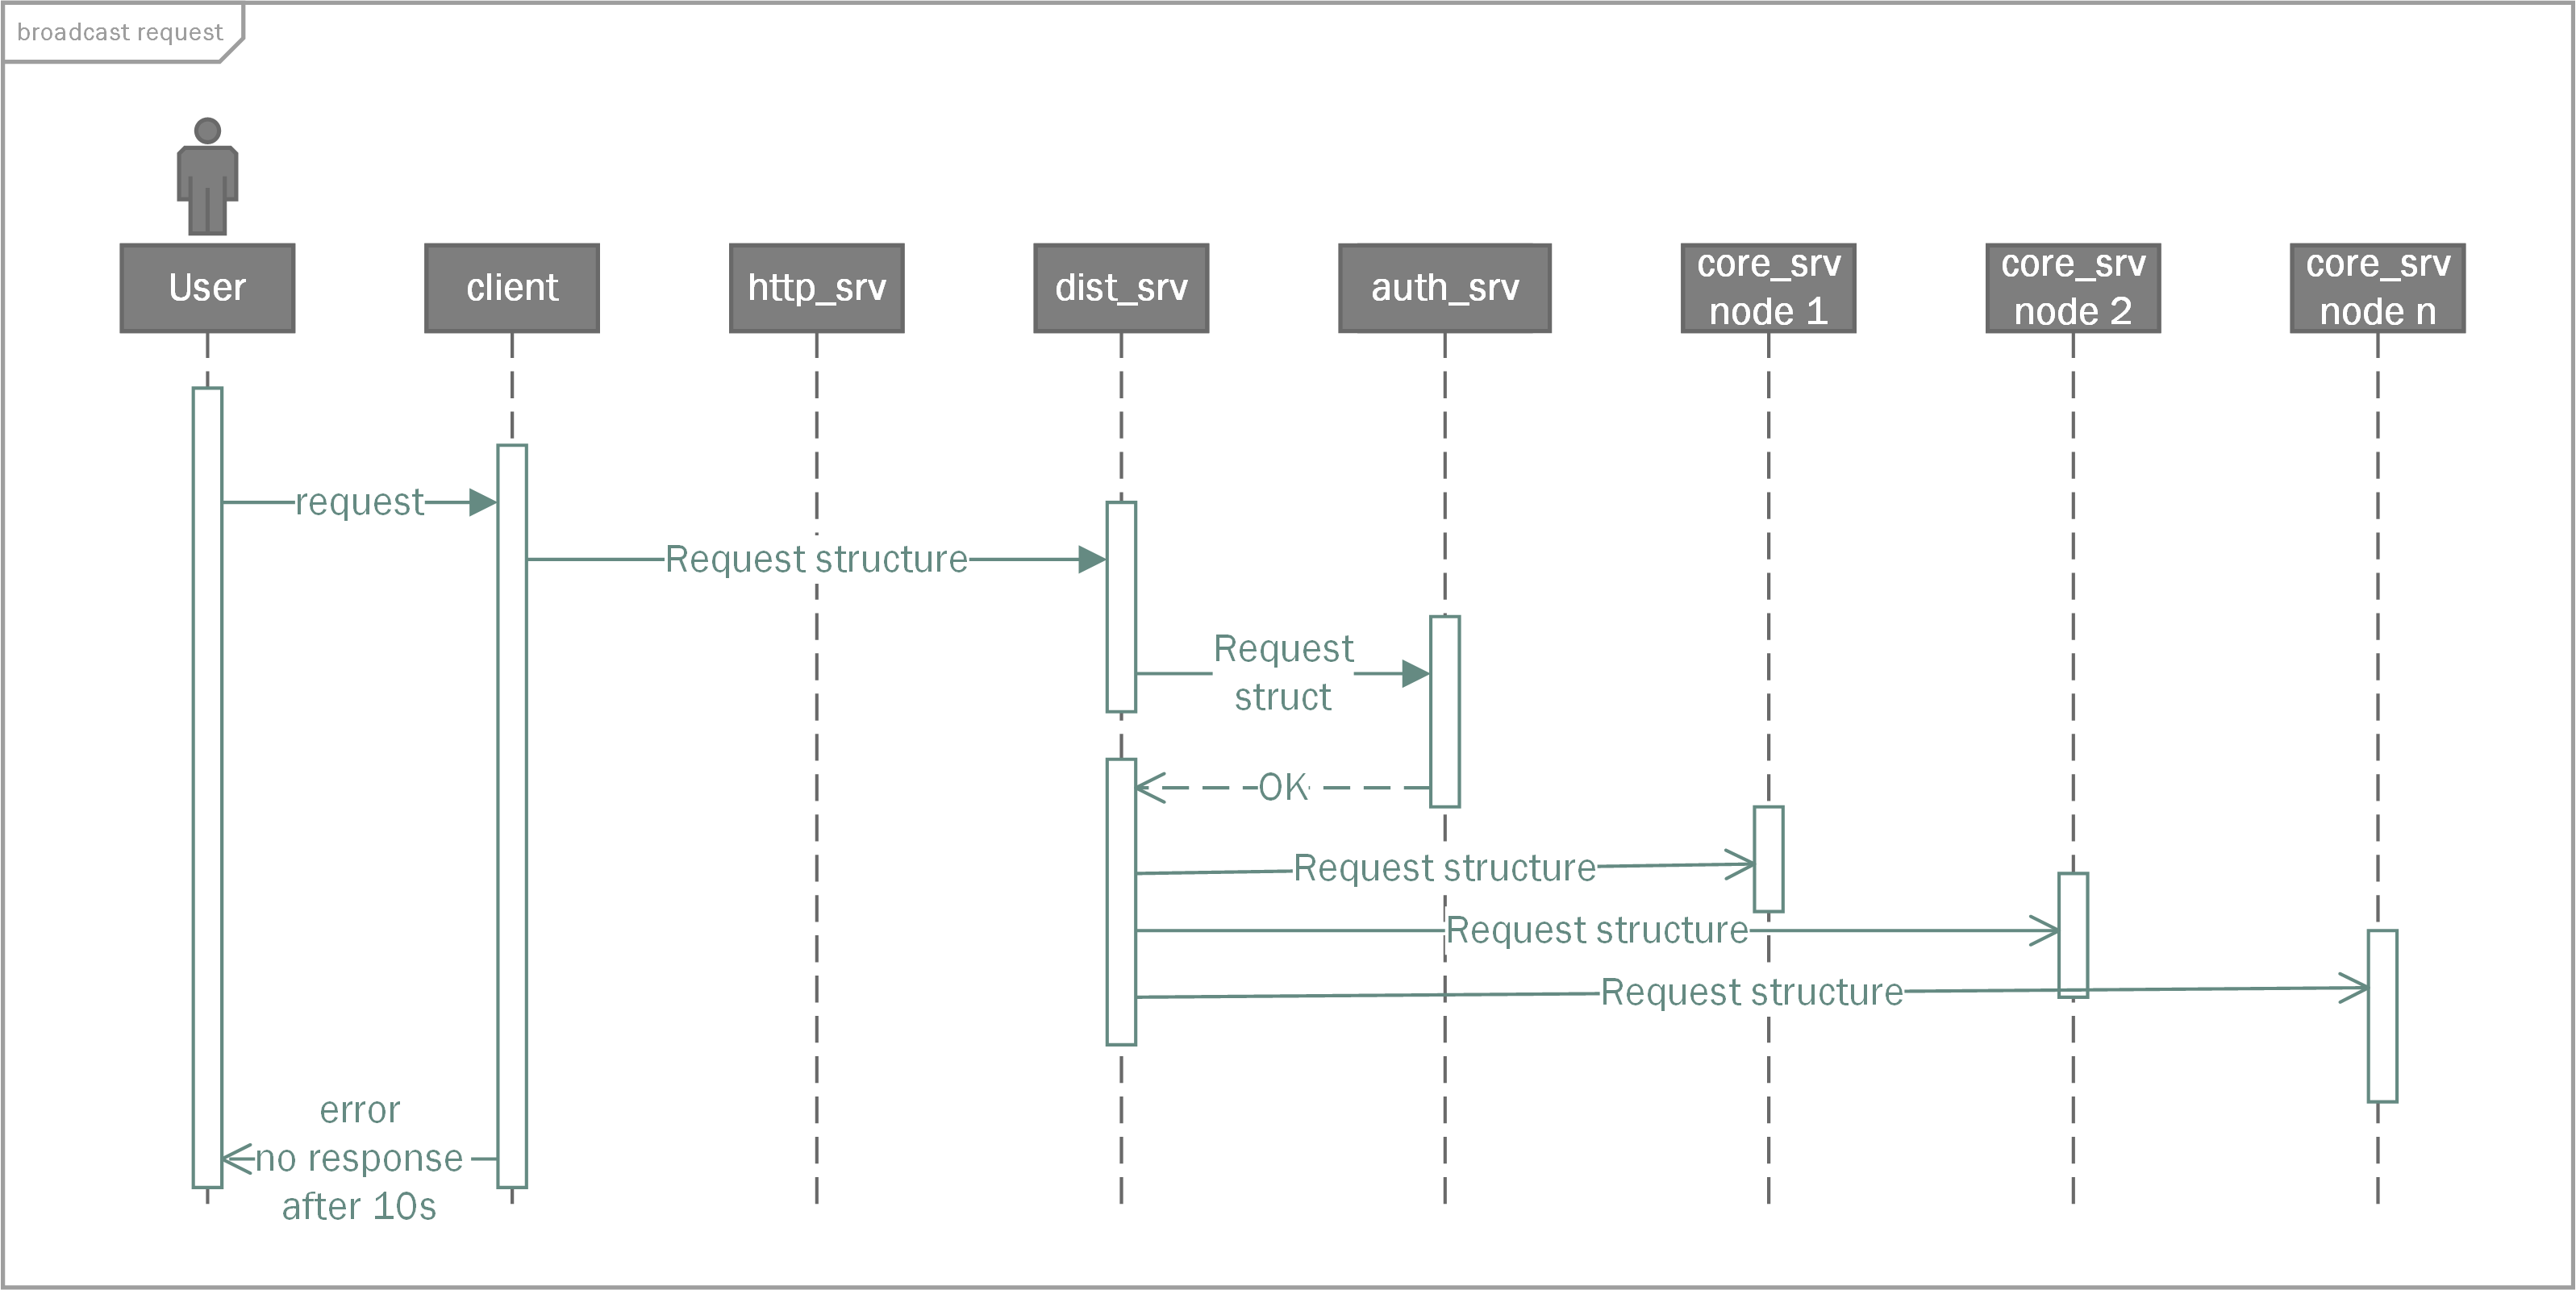
\includegraphics[width=0.9\textwidth]{broadcast-error}
	\caption[Zapytanie zakończone błędem.]{Zapytanie rozgłoszeniowe zakończone niepowodzeniem. Jeżeli biblioteka kliencka nie otrzyma przez pewien czas odpowiedzi z żadnego z węzłów, zakłada się że poszukiwany plik nie istnieje (węzeł który nie posiada szukanego pliku ignoruje zapytania).}
	\label{fig:broadcast-error}
\end{figure}

\subsubsection{Moduł HTTP}
Struktura:
\begin{itemize}
	\item storage/src/http/storage\_http\_srv.erl – gen\_server
	\item storage/src/http/http\_utils.erl – funkcje pomocnicze
\end{itemize}

Moduł służy do przetwarzania zapytań HTTP i generowania odpowiedzi. Potrafi również serwować statyczne pliki HTML – przykładowo graficzny menedżer plików.

Nie definiuje żadnego publicznego API oraz ignoruje wszystkie komunikaty pochodzące z handle\_call i handle\_cast. Jedyne dwie funkcje to standardowe start\_link() oraz stop(). Cała komunikacja z modułem dobywa się poprzez socket akceptujący połączenia na porcie określonym w pliku konfiguracyjnym.

Moduł http\_utils to zbiór funkcji pomocniczych, odpowiedzialnych za parsowanie zapytań i konstruowanie odpowiedzi HTTP. Oba moduły przedstawia\autoref{fig:http-module}.

\begin{figure}[!htbp]
	\centering
	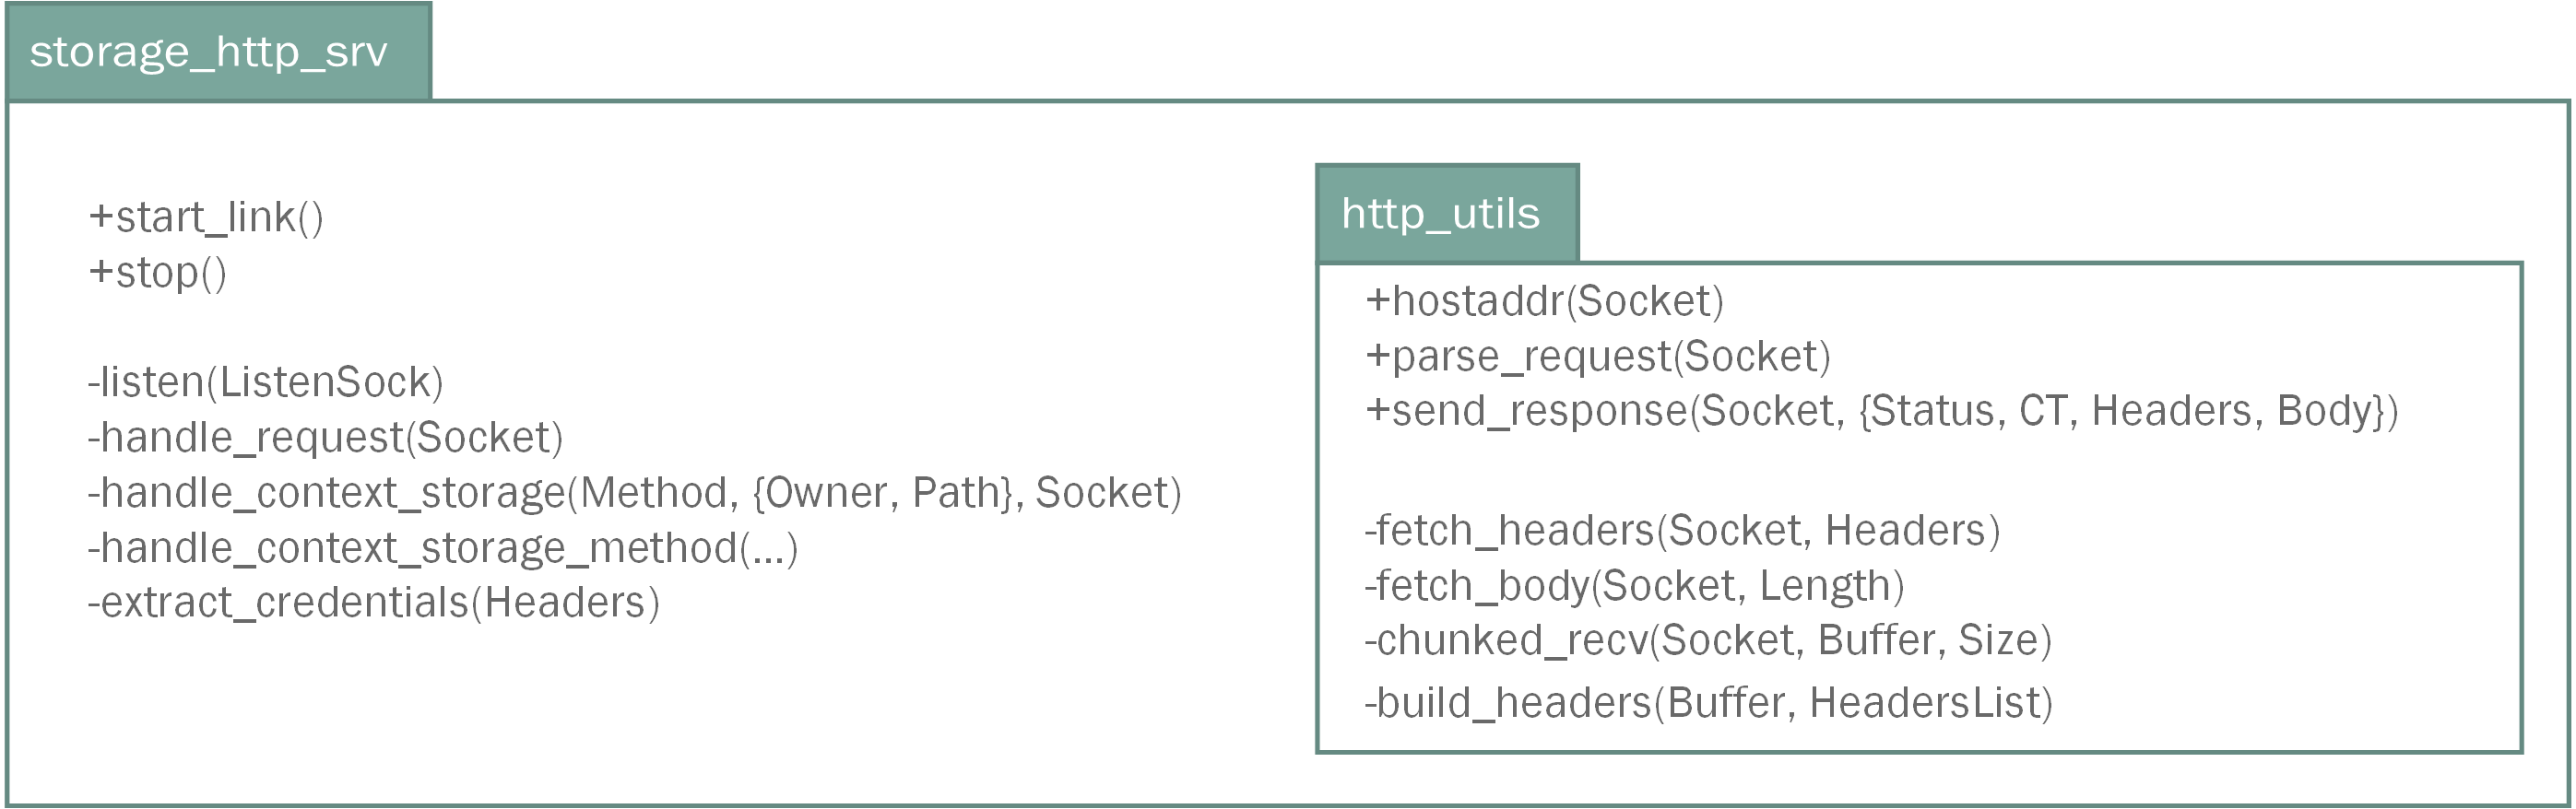
\includegraphics[width=0.9\textwidth]{http-module}
	\caption{Struktura modułu HTTP.}
	\label{fig:http-module}
\end{figure}

Budowa przykładowego zapytania, jakie można wysłać do modułu (standardowy \textit{HTTP Request}):

\begin{lstlisting}
GET storage/user02/path/to/my/file.dat HTTP/1.1
Host: ds-01.storage.example.com:9001
Authorization: HMAC user01:6c51adc384572536d9c8a9dbcfbebf590942771f
\end{lstlisting}

Zostanie przetłumaczone na poniższą strukturę Request:

\begin{lstlisting}
-record(request, {
	type 		= 'read', 
	user 		= "user01"
	addr 		= {"user02", " path/to/my/file.dat},
	hmac 		= "6c51adc384572536d9c8a9dbcfbebf590942771f", 
	data 		= none, 
	opts 		= none 
}).
\end{lstlisting}

Jeżeli plik zostanie znaleziony a użytkownik będzie mógł go odczytać, serwer zwróci odpowiedź HTTP 200 OK, a w treści znajdzie się zawartość binarna pliku.

Diagram sekwencji obsługi przykładowego zapytania typu GET (odczyt pliku) przedstawia \autoref{fig:http-seq}.

\begin{figure}[!htbp]
	\centering
	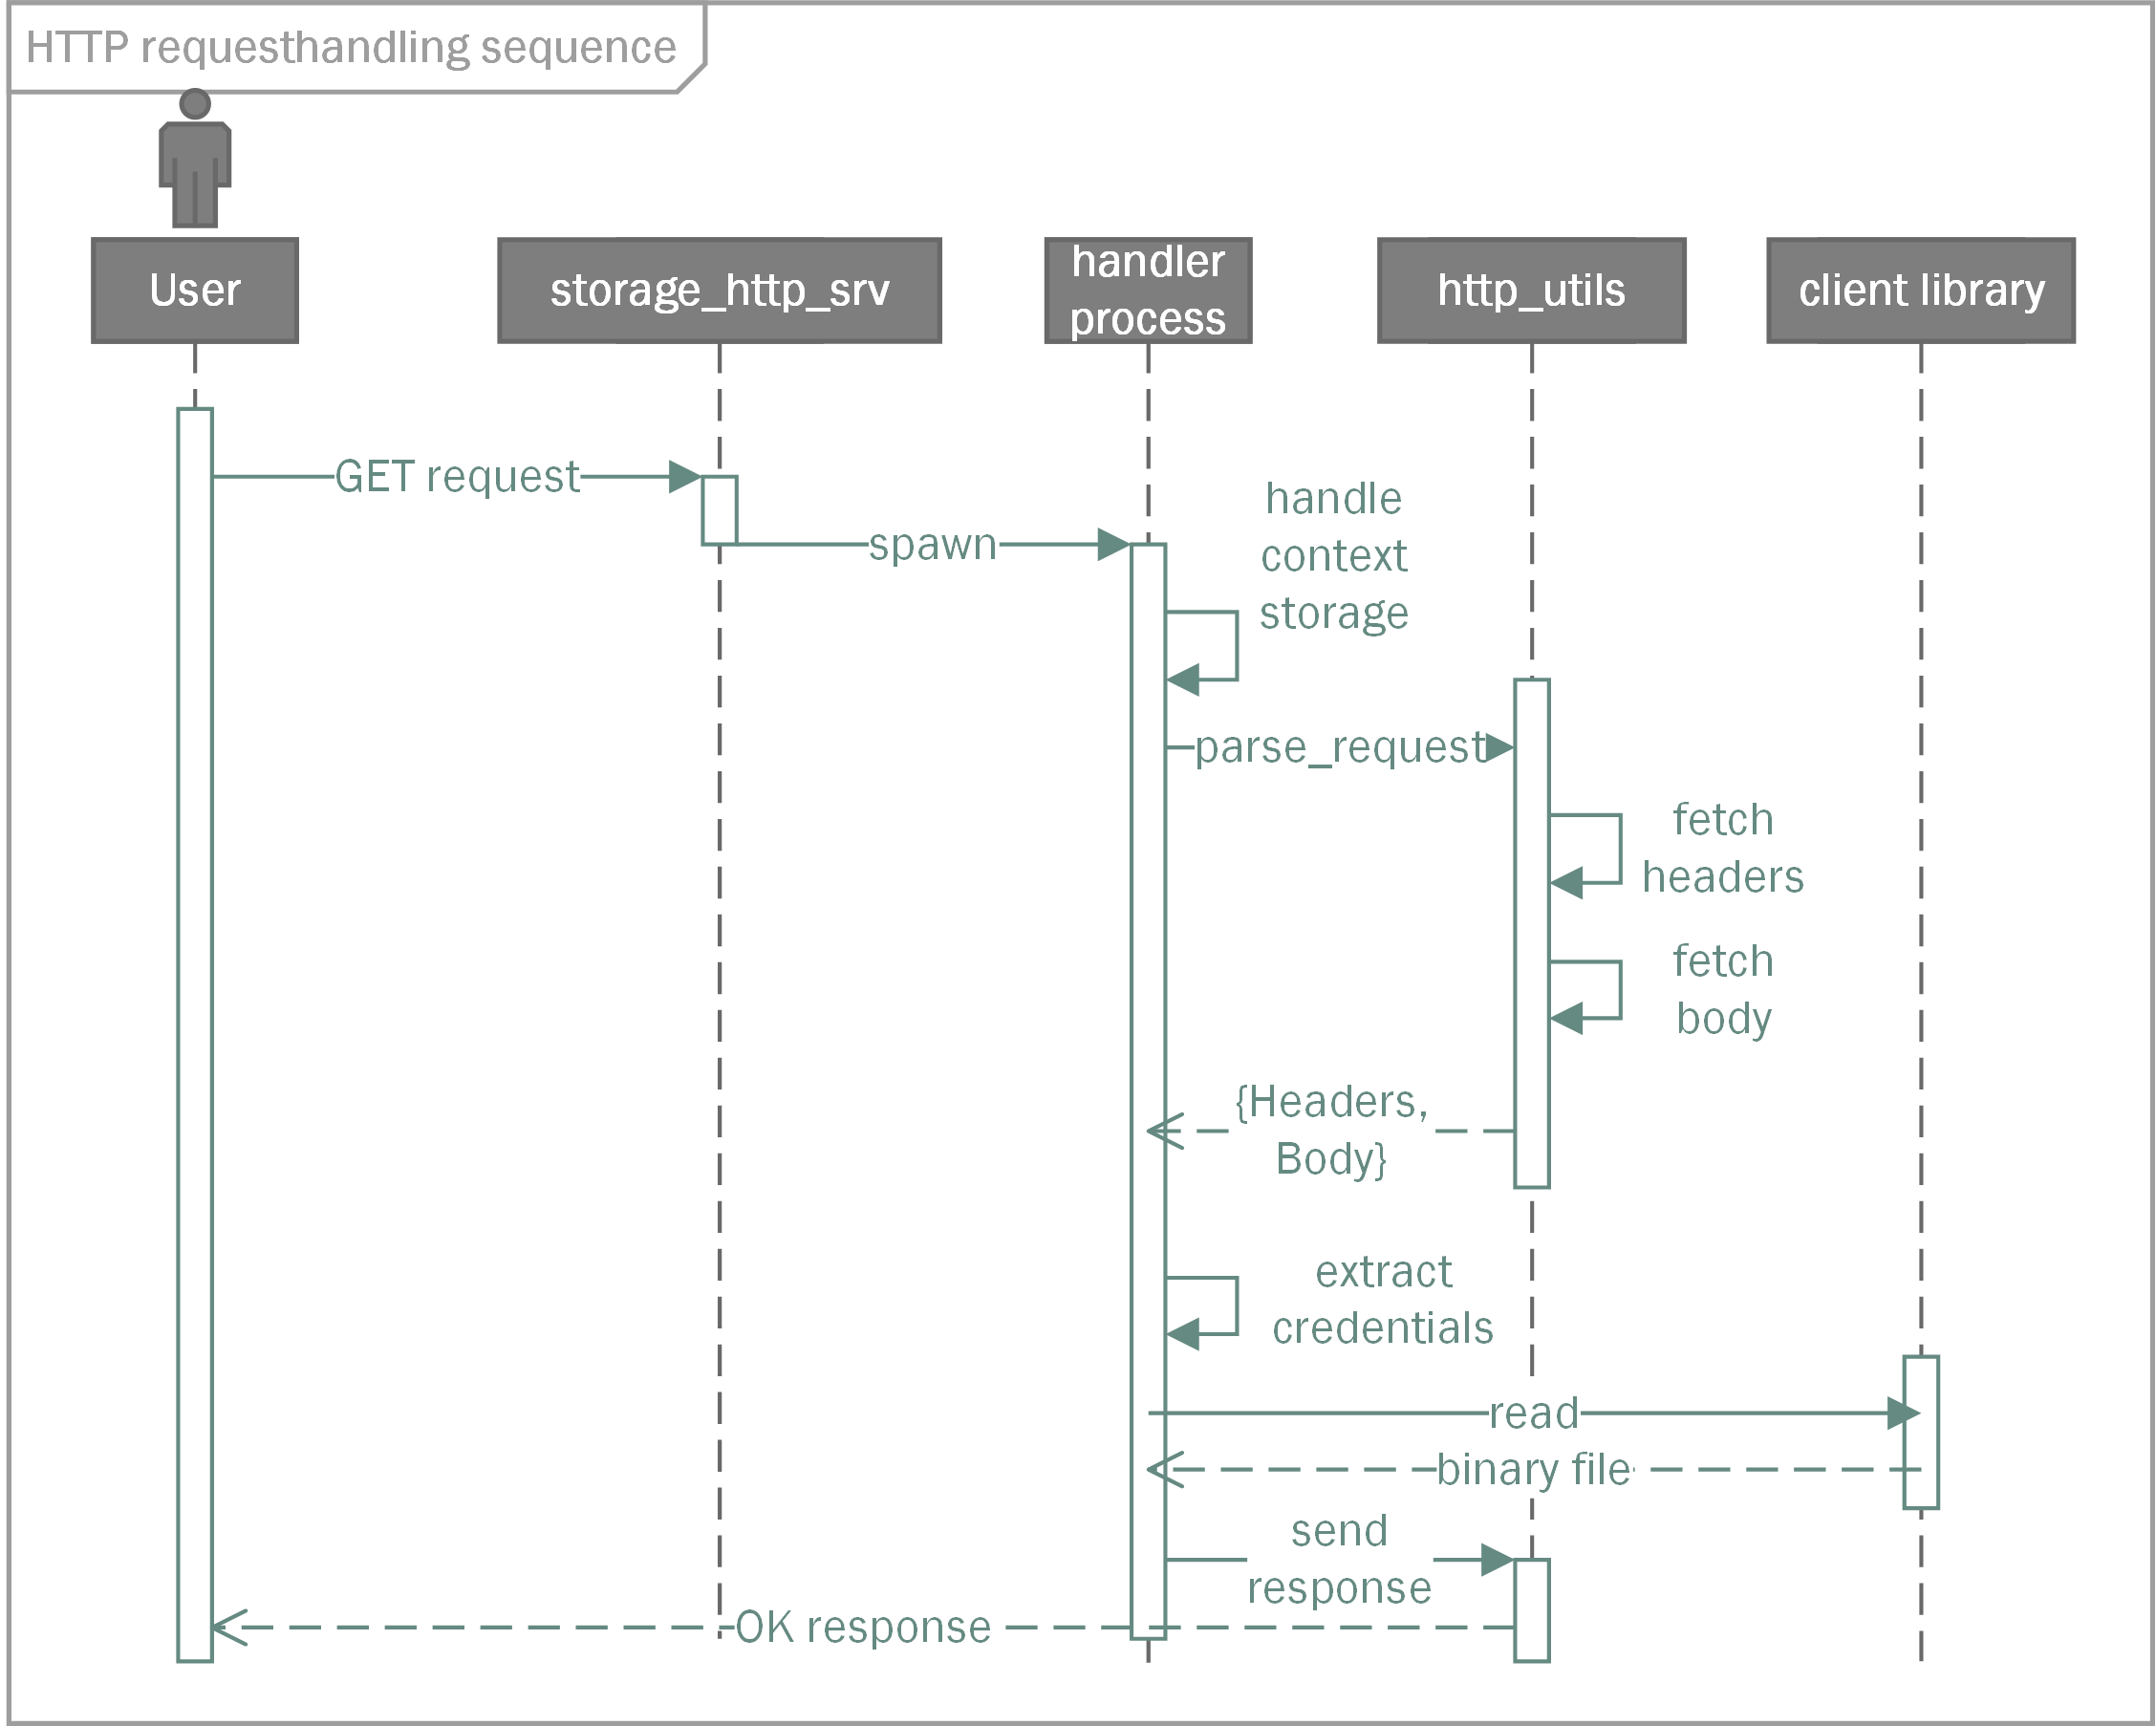
\includegraphics[width=0.9\textwidth]{http-seq}
	\caption[Przetwarzanie zapytania w module HTTP]{Przetwarzanie zapytania HTTP w module storage\_http\_srv. Dla każdego zapytania uruchamiany jest osobny wątek odpowiedzialny za jego obsługę, który parsuje zapytanie, wykonuje żądaną akcję przy użyciu biblioteki klienckiej a rezultat zwraca z powrotem przy użyciu protokołu HTTP.}
	\label{fig:http-seq}
\end{figure}
\subsubsection{Moduł autentykacji}
Struktura:
\begin{itemize}
	\item storage/src/auth/storage\_auth\_srv.erl – gen\_server
	\item storage/src/auth/db\_users.erl – DAO dla struktur User
\end{itemize}

Moduł autentykacji odpowiada za obliczanie i weryfikację sumy kontrolnej HMAC przekazywanych zapytań. Moduł db\_users jest modułem dostępowym do encji reprezentujących użytkownika (struktury User), przechowywanych w bazie danych. Suma HMAC opisana jest dokładniej w kolejnym punkcie.

\begin{figure}[!htbp]
	\centering
	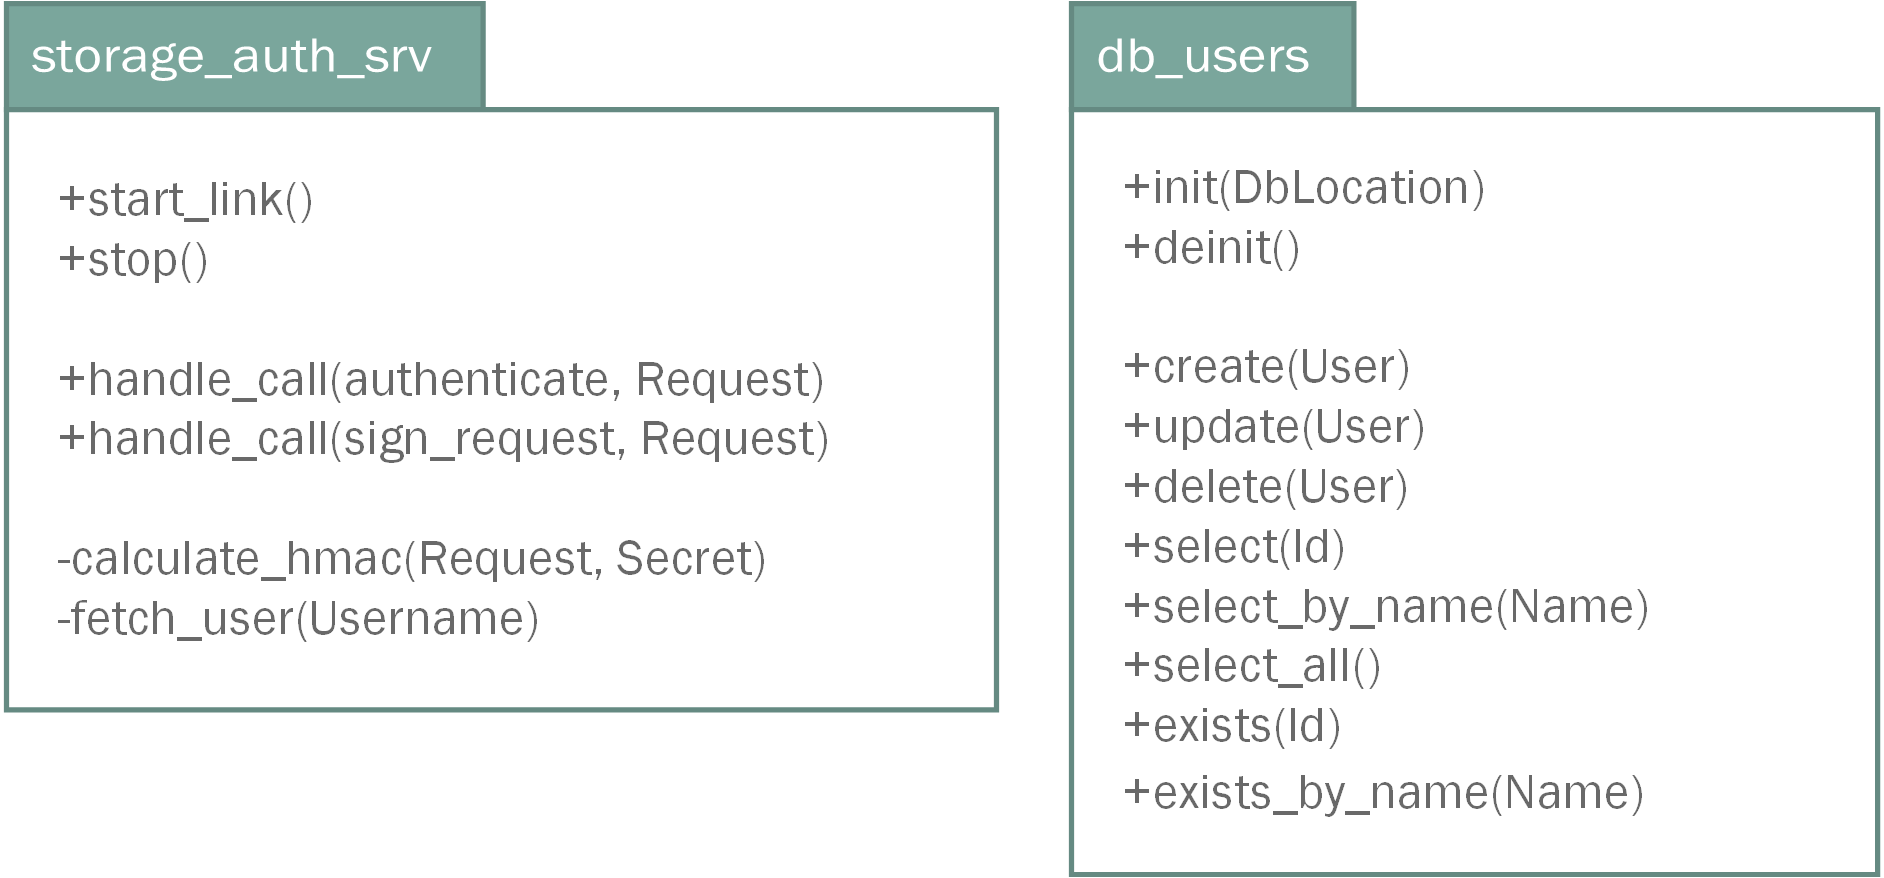
\includegraphics[width=0.9\textwidth]{auth-module}
	\caption[Budowa modułu autentykacji.]{Moduły składające się na moduł autentykacji. storage\_auth\_srv pozwala na porównanie sumy kontrolnej otrzymanego zapytania z wartością, którą sam wylicza. db\_users oferuje podstawowe operacje na bazie użytkowników, z wykorzystaniem struktury User.}
	\label{fig:auth-module}
\end{figure}

Serwer storage\_auth\_srv przechowuje tablicę ets zawierającą krotki {Username, Secret, Expires}, pełniącą rolę pamięci podręcznej. Znajdują się w niej użytkownicy wraz z ich kluczami prywatnymi. Opis aktualizacji tej tablicy znajduje się w rozdziale Synchronizacja użytkowników.

\paragraph{Suma HMAC:} keyed-Hash Message Authentication Code to funkcja skrótu z dodatkowo wmieszanym kluczem prywatnym. Wynikowy kod zależy nie tylko od danych z których jest obliczany, ale również od wykorzystanego hasła. Hasło (klucz prywatny) znane jest tylko użytkownikowi oraz systemowi. Nie jest przesyłane między nimi, co zmniejsza szanse na ujawnienie klucza.

Wykorzystanie HMAC zapewnia ochronę integralności przesyłanych zapytań (modyfikacja parametrów zapytania wymaga przeliczenia sumy HMAC) oraz autentyczności danych (wyliczenie sumy wymaga znajomości klucza prywatnego).

Każdy użytkownik posiada "hasło". Może on je ustalić dowolnie ze swoimi preferencjami. Kluczem prywatnym staje się suma SHA1 obliczona z tego hasła, i tylko ta wartość przechowywana jest w bazie danych.

\subsubsection{Moduł komunikacyjny}
Struktura:
\begin{itemize}
	\item storage/src/dist/storage\_dist\_srv.erl – gen\_server
\end{itemize}
Jest to moduł odpowiedzialny za komunikację między węzłami systemu. Zapytania generowane przez bibliotekę kliencką trafiają właśnie tutaj. Są autentykowane a następnie przesyłane dalej zgodnie z polityką obsługi danego typu zapytania.

gen\_server w swoim stanie przechowuje zbiór adresów wszystkich węzłów w systemie (rezultat wywołania node() na każdym węźle). Standardowy protokół tworzenia i aktualizacji tego zbioru opisuje rozdział Dołączanie węzłów (synchronizacja stanu).

\begin{figure}[!htbp]
	\centering
	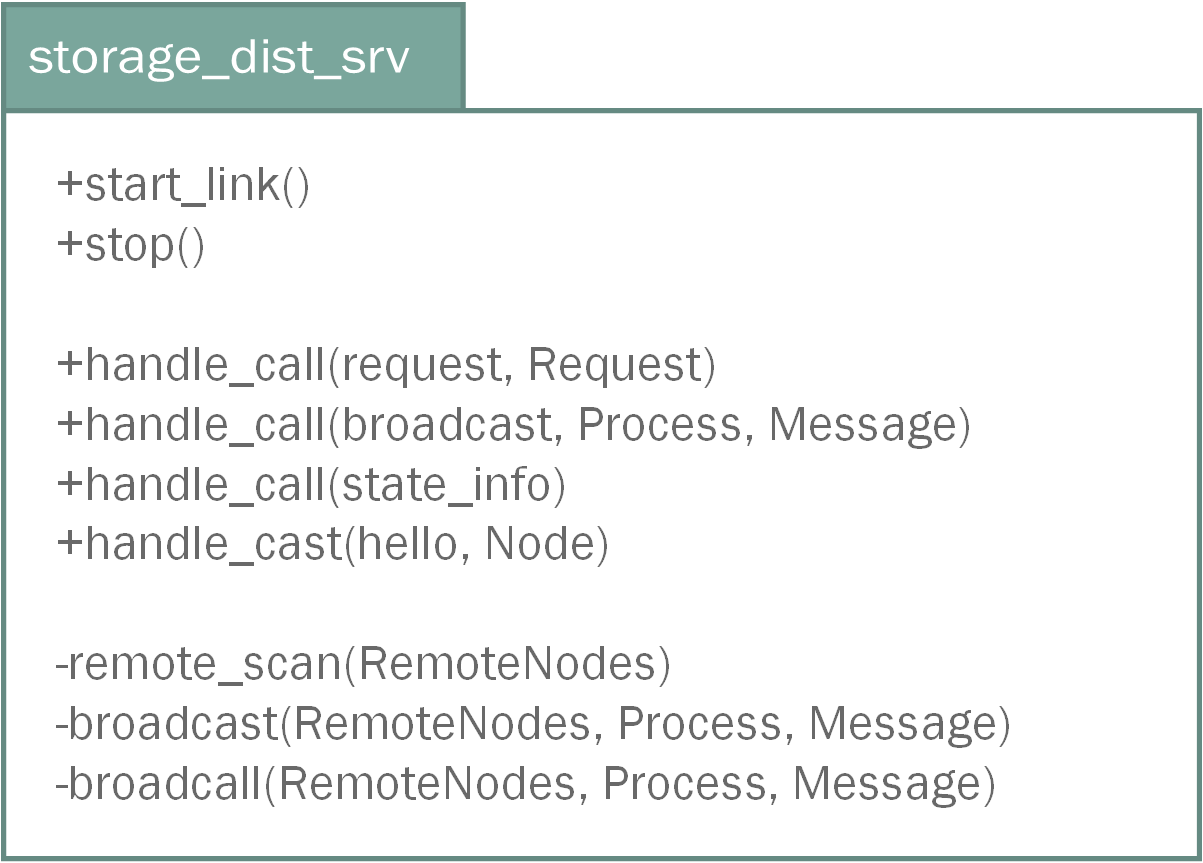
\includegraphics[width=0.7\textwidth]{dist-module}
	\caption[Struktura modułu komunikacyjnego.]{Publiczny interfejs modułu storage\_dist\_srv. Podstawowa metoda to handle\_call(request, Request), która jest zdalnie wywoływana przez API klienckie z odpowiednią strukturą zapytania jako argument.}
	\label{fig:dist-module}
\end{figure}

\paragraph{Obsługa zapytań read, delete, find} Wszystkie te zapytania obsługiwane są w identyczny sposób. Przykładowy ciąg sekwencji przy obsłudze zapytania typu read (rozsyłanego do wszystkich węzłów) przedstawia \autoref{fig:dist-seq}.

Źródłem zapytania jest proces używający biblioteki klienckiej (client), wywołujący synchroniczne zapytanie na module storage\_dist\_srv. Od razu tworzony jest nowy proces odpowiedzialny za obsługę tego żądania. Główny proces gen\_servera zwraca z handle\_call status noreply i kontynuuje działanie. Wygenerowanie odpowiedzi i przesłanie jej do użytkownika będzie należało do jednego z modułów storage\_core\_srv, gdzie przesłana jest odpowiednia struktura Request.

Proces obsługi zapytania autentykuje je przy użyciu modułu storage\_auth\_srv zaraz po jego otrzymaniu.

\begin{figure}[!htbp]
	\centering
	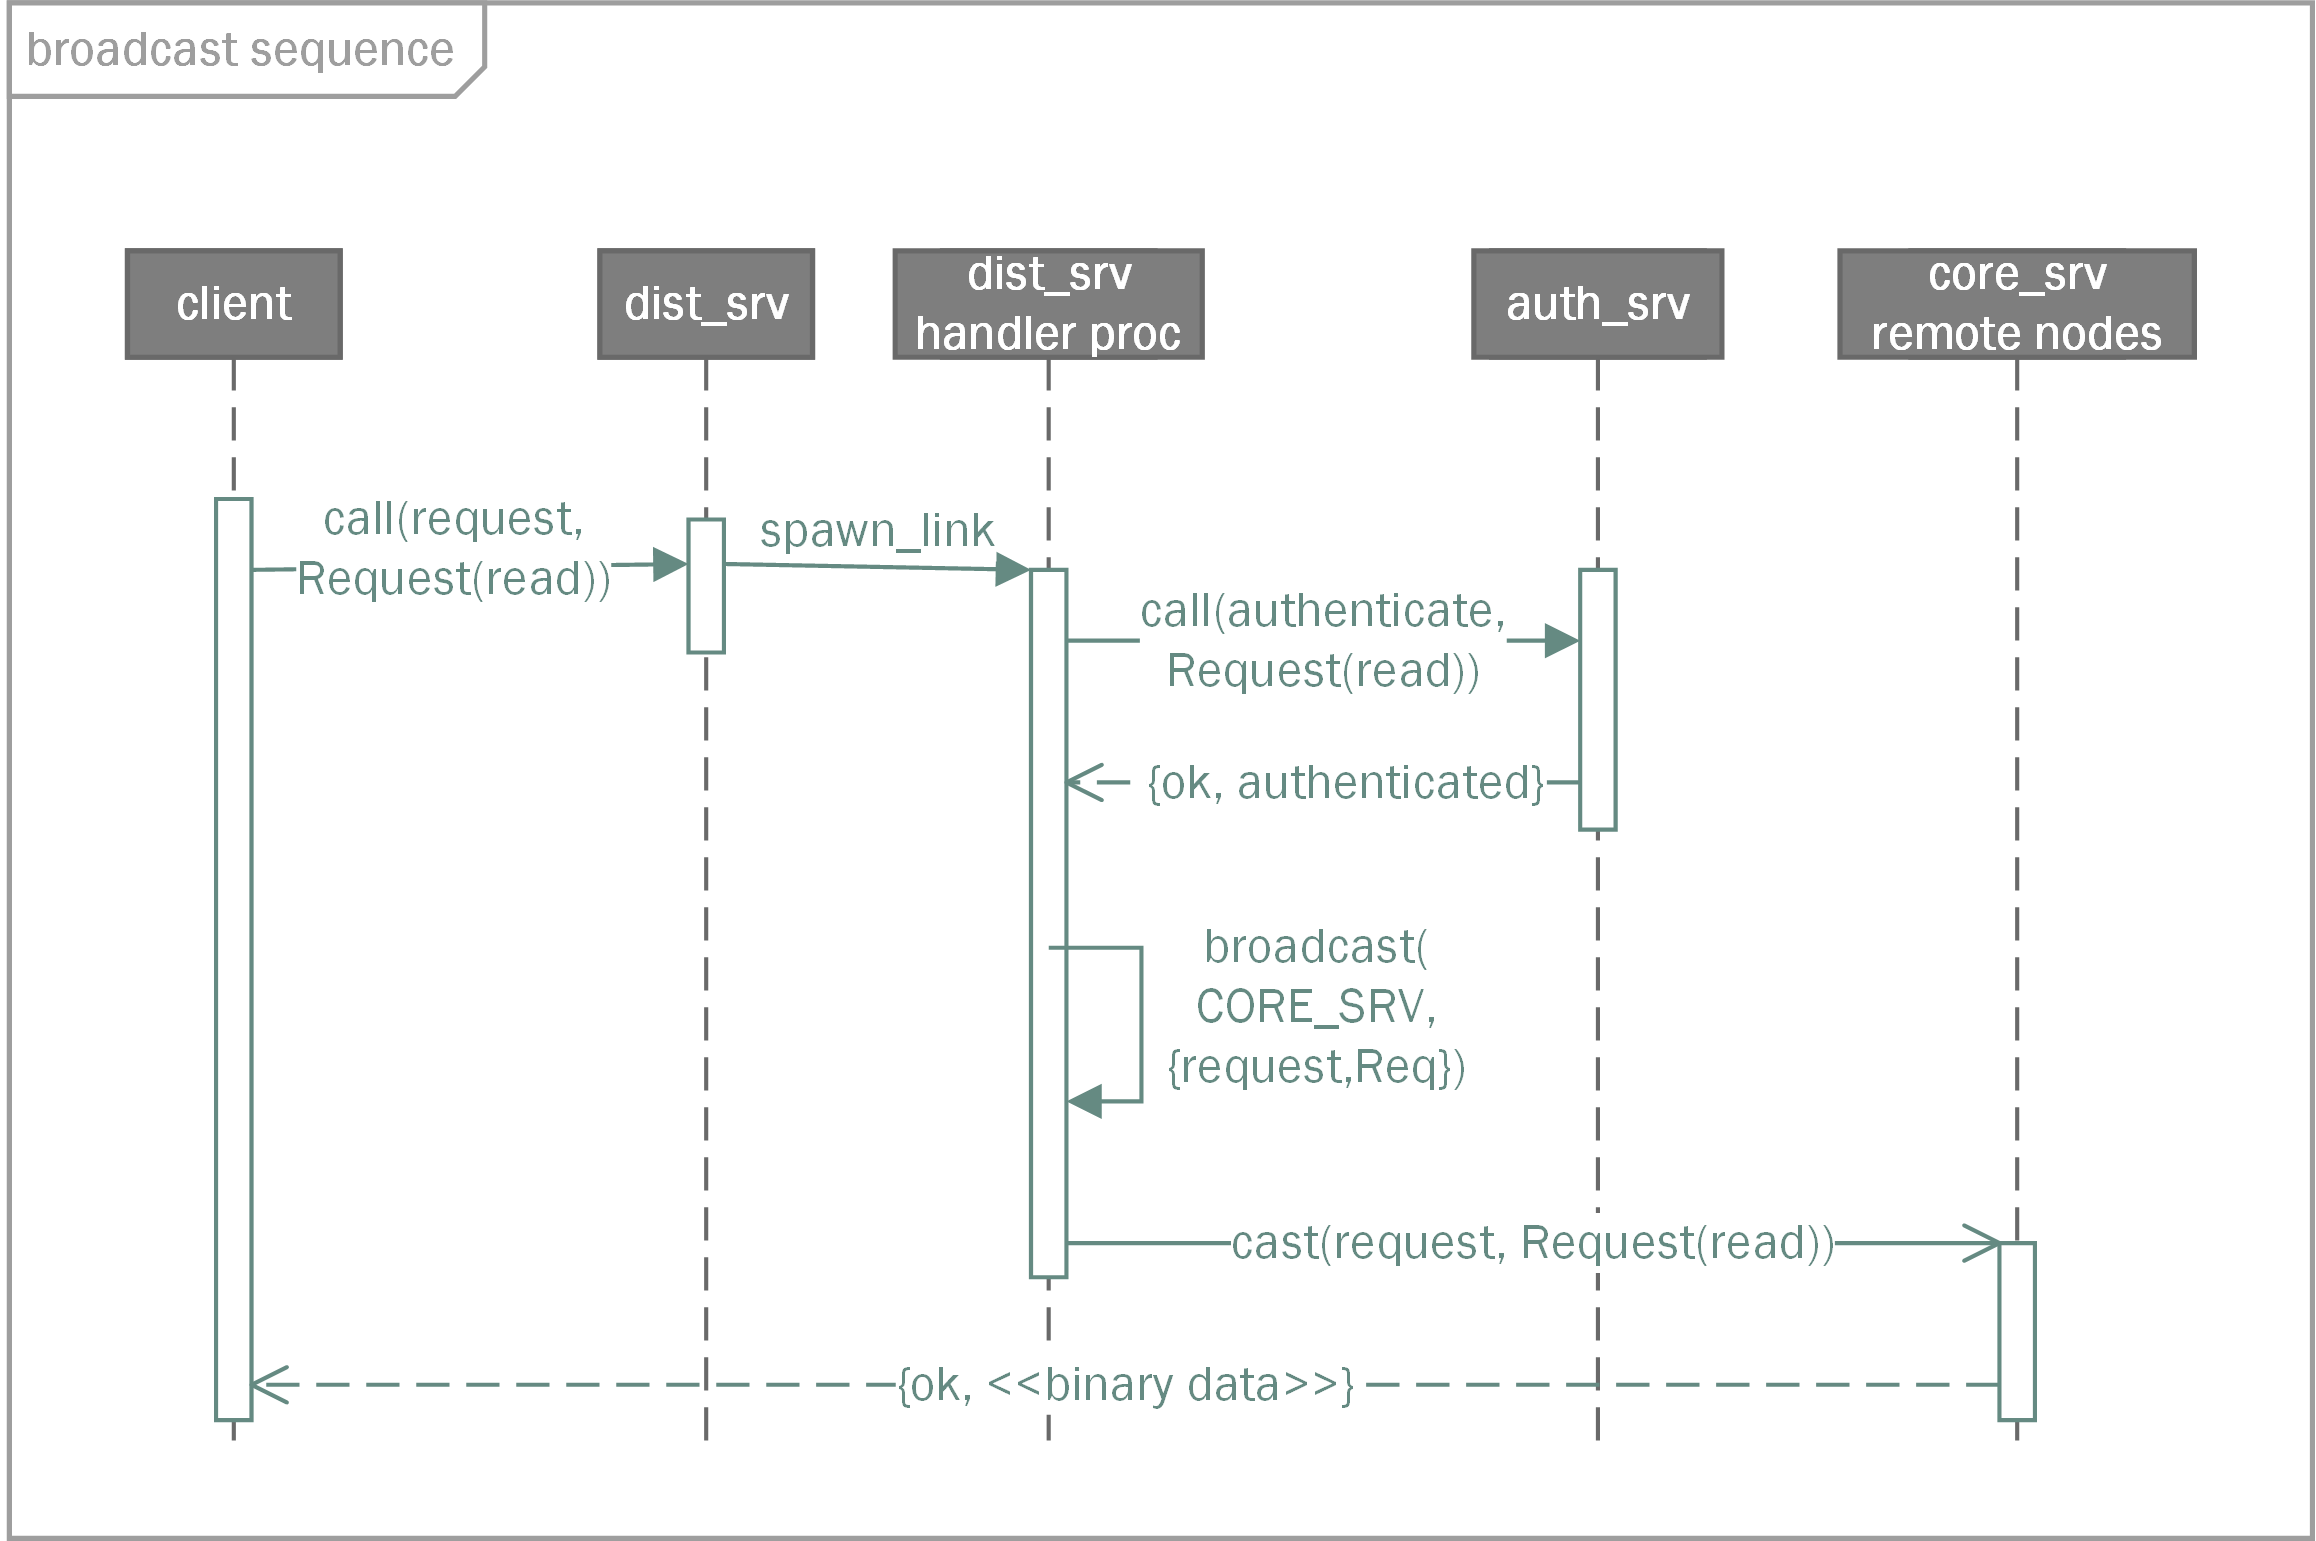
\includegraphics[width=0.9\textwidth]{dist-seq}
	\caption[Zapytanie \textit{read} w module komunikacyjnym.]{Sekwencja wywołań przy obsłudze zapytania read w module storage\_dist\_srv.}
	\label{fig:dist-seq}
\end{figure}

\paragraph{Obsługa zapytań create}
Zapytanie create różni się od obsługi zapytań read, delete czy find. Wymaga zlokalizowania węzła o najmniejszym zapełnieniu, który może pomieścić dany plik. Do modułów storage\_core\_srv na wszystkich węzłach w systemie wysyłana jest wiadomość {reserve, Size}, gdzie Size jest rozmiarem pliku. Jeżeli dany węzeł może przyjąć plik, odpowiada komunikatem {ok, Fill}, gdzie Fill jest jego procentowym zapełnieniem. Do niego następnie przesyłane jest właściwe żądanie użytkownika. Do pozostałych węzłów trafia komunikat {release, Size}, mówiący, że mogą zwolnić zarezerwowane zasoby dyskowe. Sekwencja wywołań przedstawiona jest na \autoref{fig:dist-create-seq}.

\begin{figure}[!htbp]
	\centering
	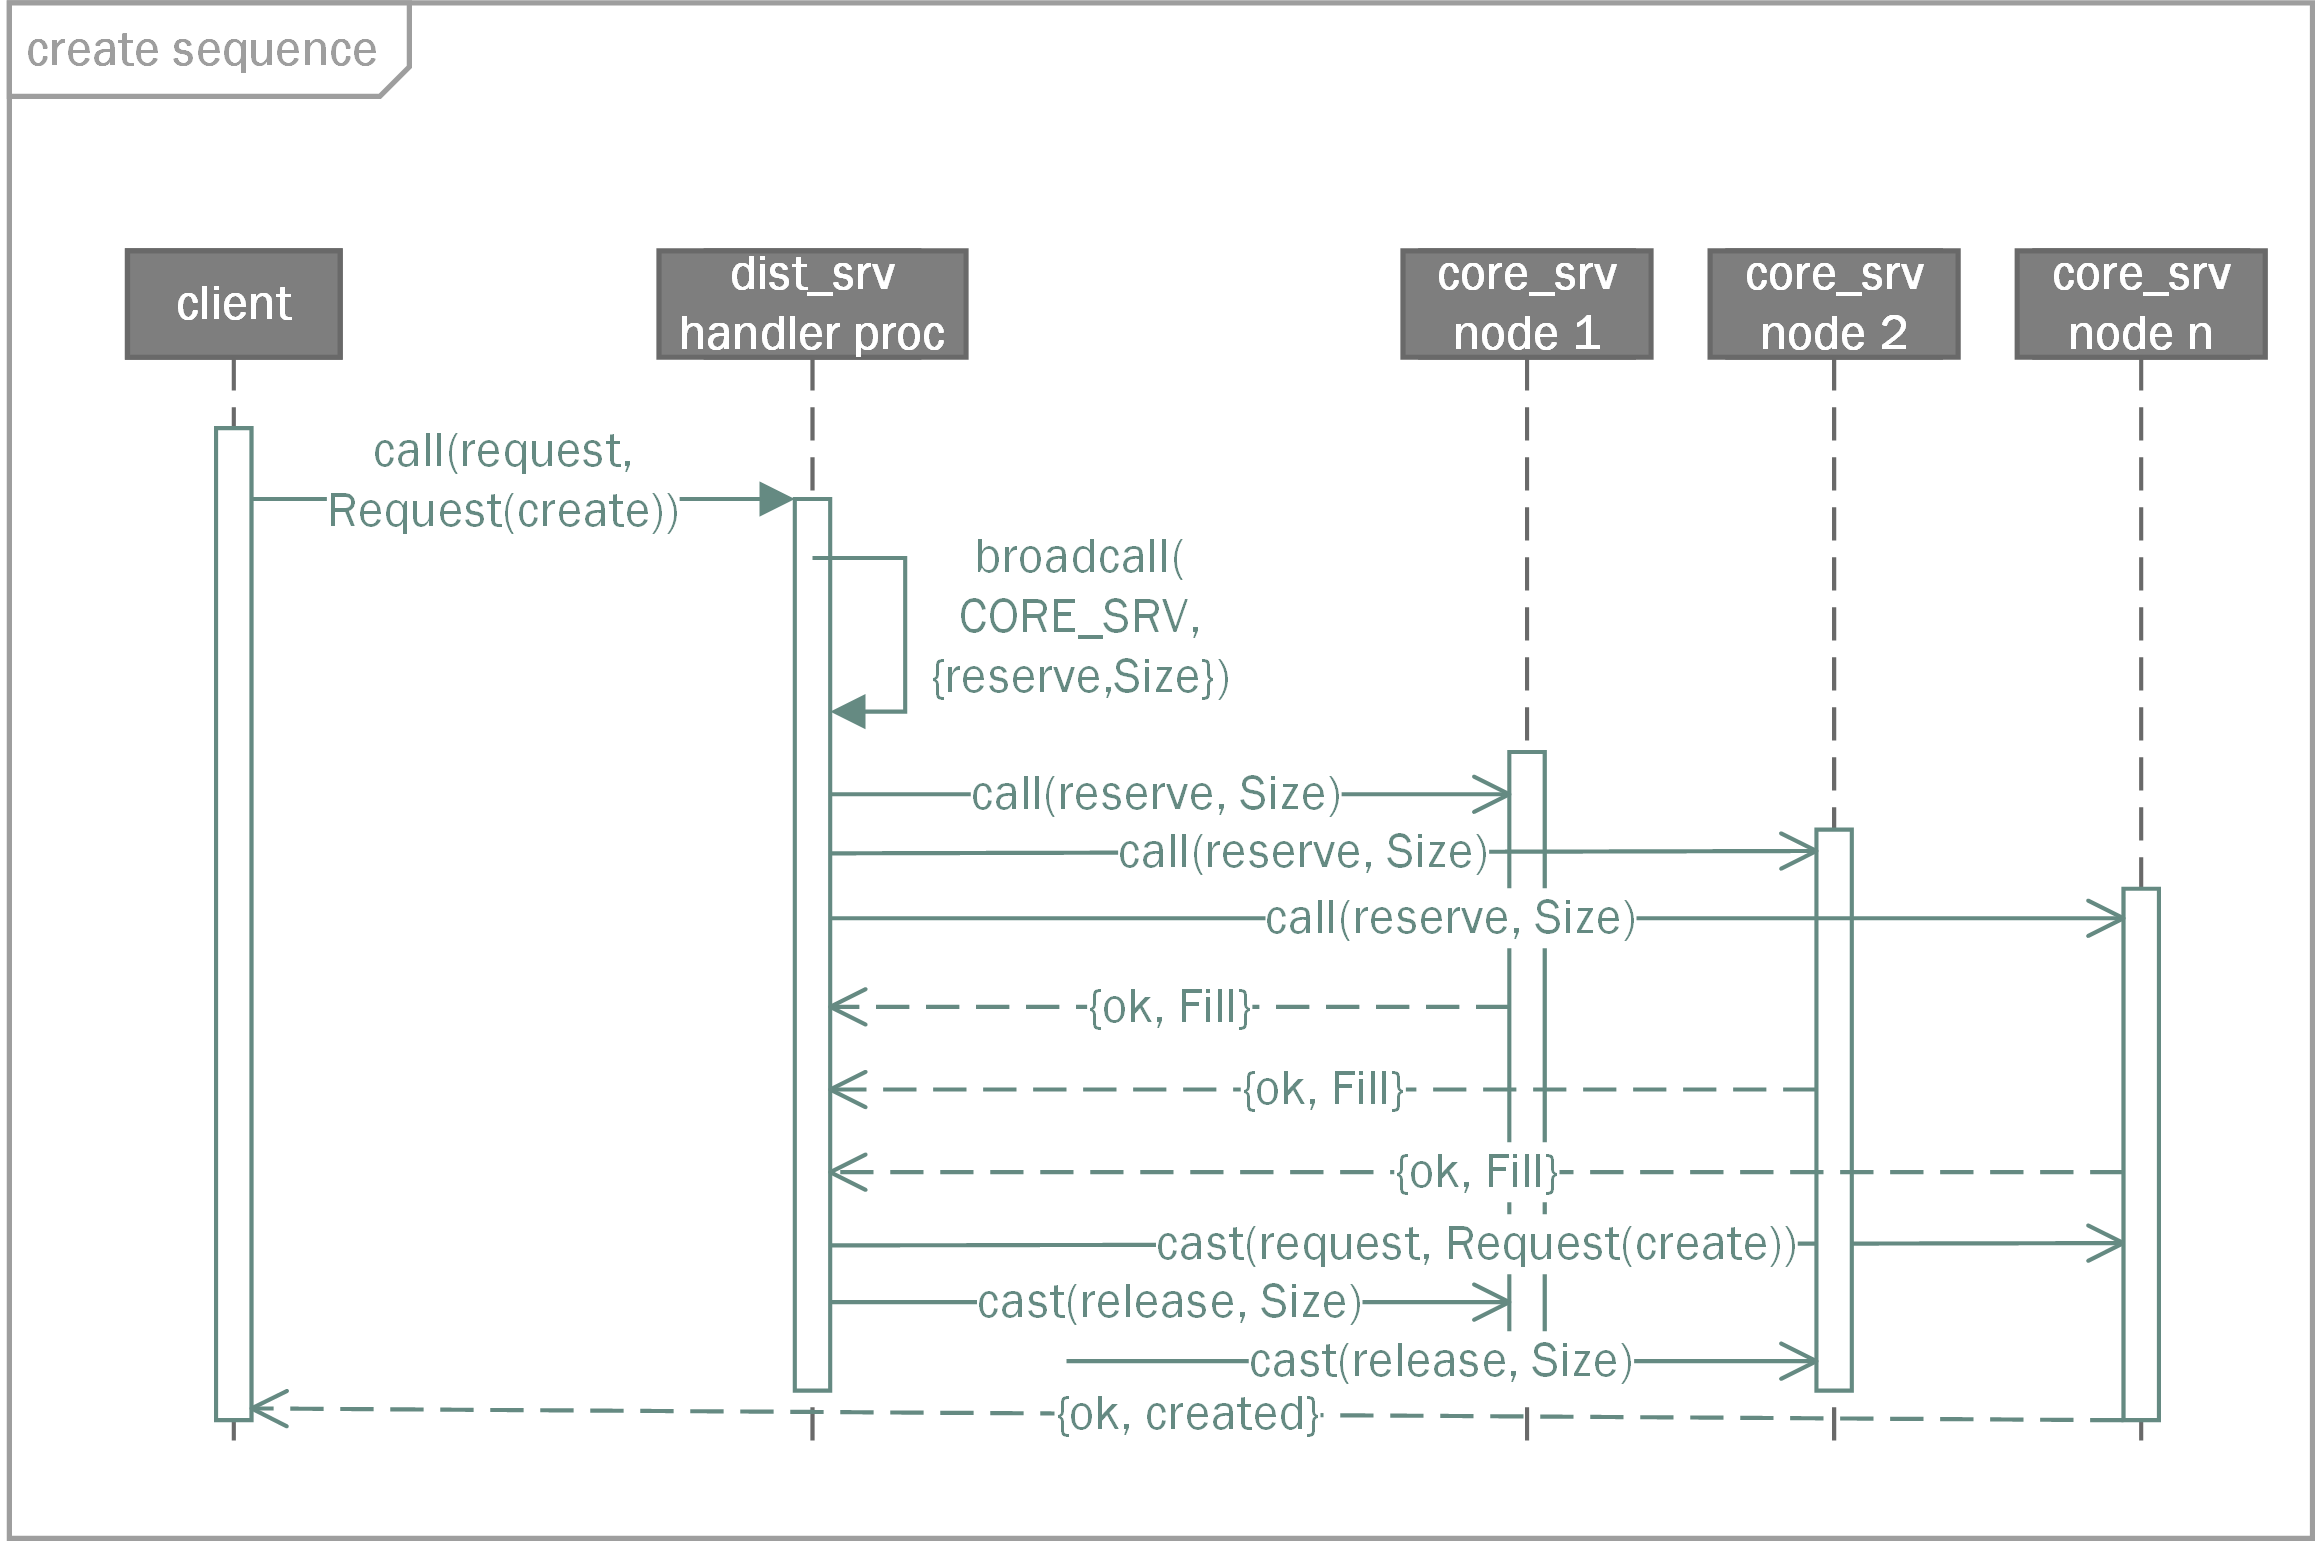
\includegraphics[width=0.9\textwidth]{dist-create-seq}
	\caption[Zapytanie \textit{create} w module komunikacyjnym.]{Obsługa zapytania create. Następuje rezerwacja miejsca na wszystkich węzłach, wybierany jest najbardziej odpowiedni do przechowania pliku, a zarezerwowane miejsce jest zwalniane.}
	\label{fig:dist-create-seq}
\end{figure}


\paragraph{Obsługa zapytań update}
Zapytanie update przekazywane jest bezpośrednio do węzła który przechowuje aktualizowany plik. Implementacja wykorzystuje dodatkowe zapytanie find, w celu zlokalizowania tego węzła. Sekwencja jest więc bardzo podobna do tej przedstawionej na \autoref{fig:dist-seq}.

\subsubsection{Moduł wykonawczy}
Struktura:
\begin{itemize}
	\item storage/src/core/storage\_core\_srv.erl – gen\_server
\item storage/src/core/db\_files.erl – DAO dla struktur File
\item storage/src/core/db\_actions.erl – DAO dla struktur Action
\item storage/src/core/core.erl – implementacja operacji plikowych
\item storage/src/core/files.erl – funkcje I/O
\item storage/src/core/scheduler.erl – scheduler i wątki wykonawcze
\end{itemize}

Moduł core to główny moduł systemu, odpowiedzialny za realizację wszystkich zleconych operacji. Komunikuje się bezpośrednio z bazą danych i systemem plików. Tutaj trafiają wszystkie zapytania w finalnej fazie obsługi. Odpowiedzi kierowane są zwykle wprost do użytkownika.

Składowe moduł i zawartość każdego z nich przedstawia diagram pokazany na \autoref{fig:core-module}.

\begin{figure}[!htbp]
	\centering
	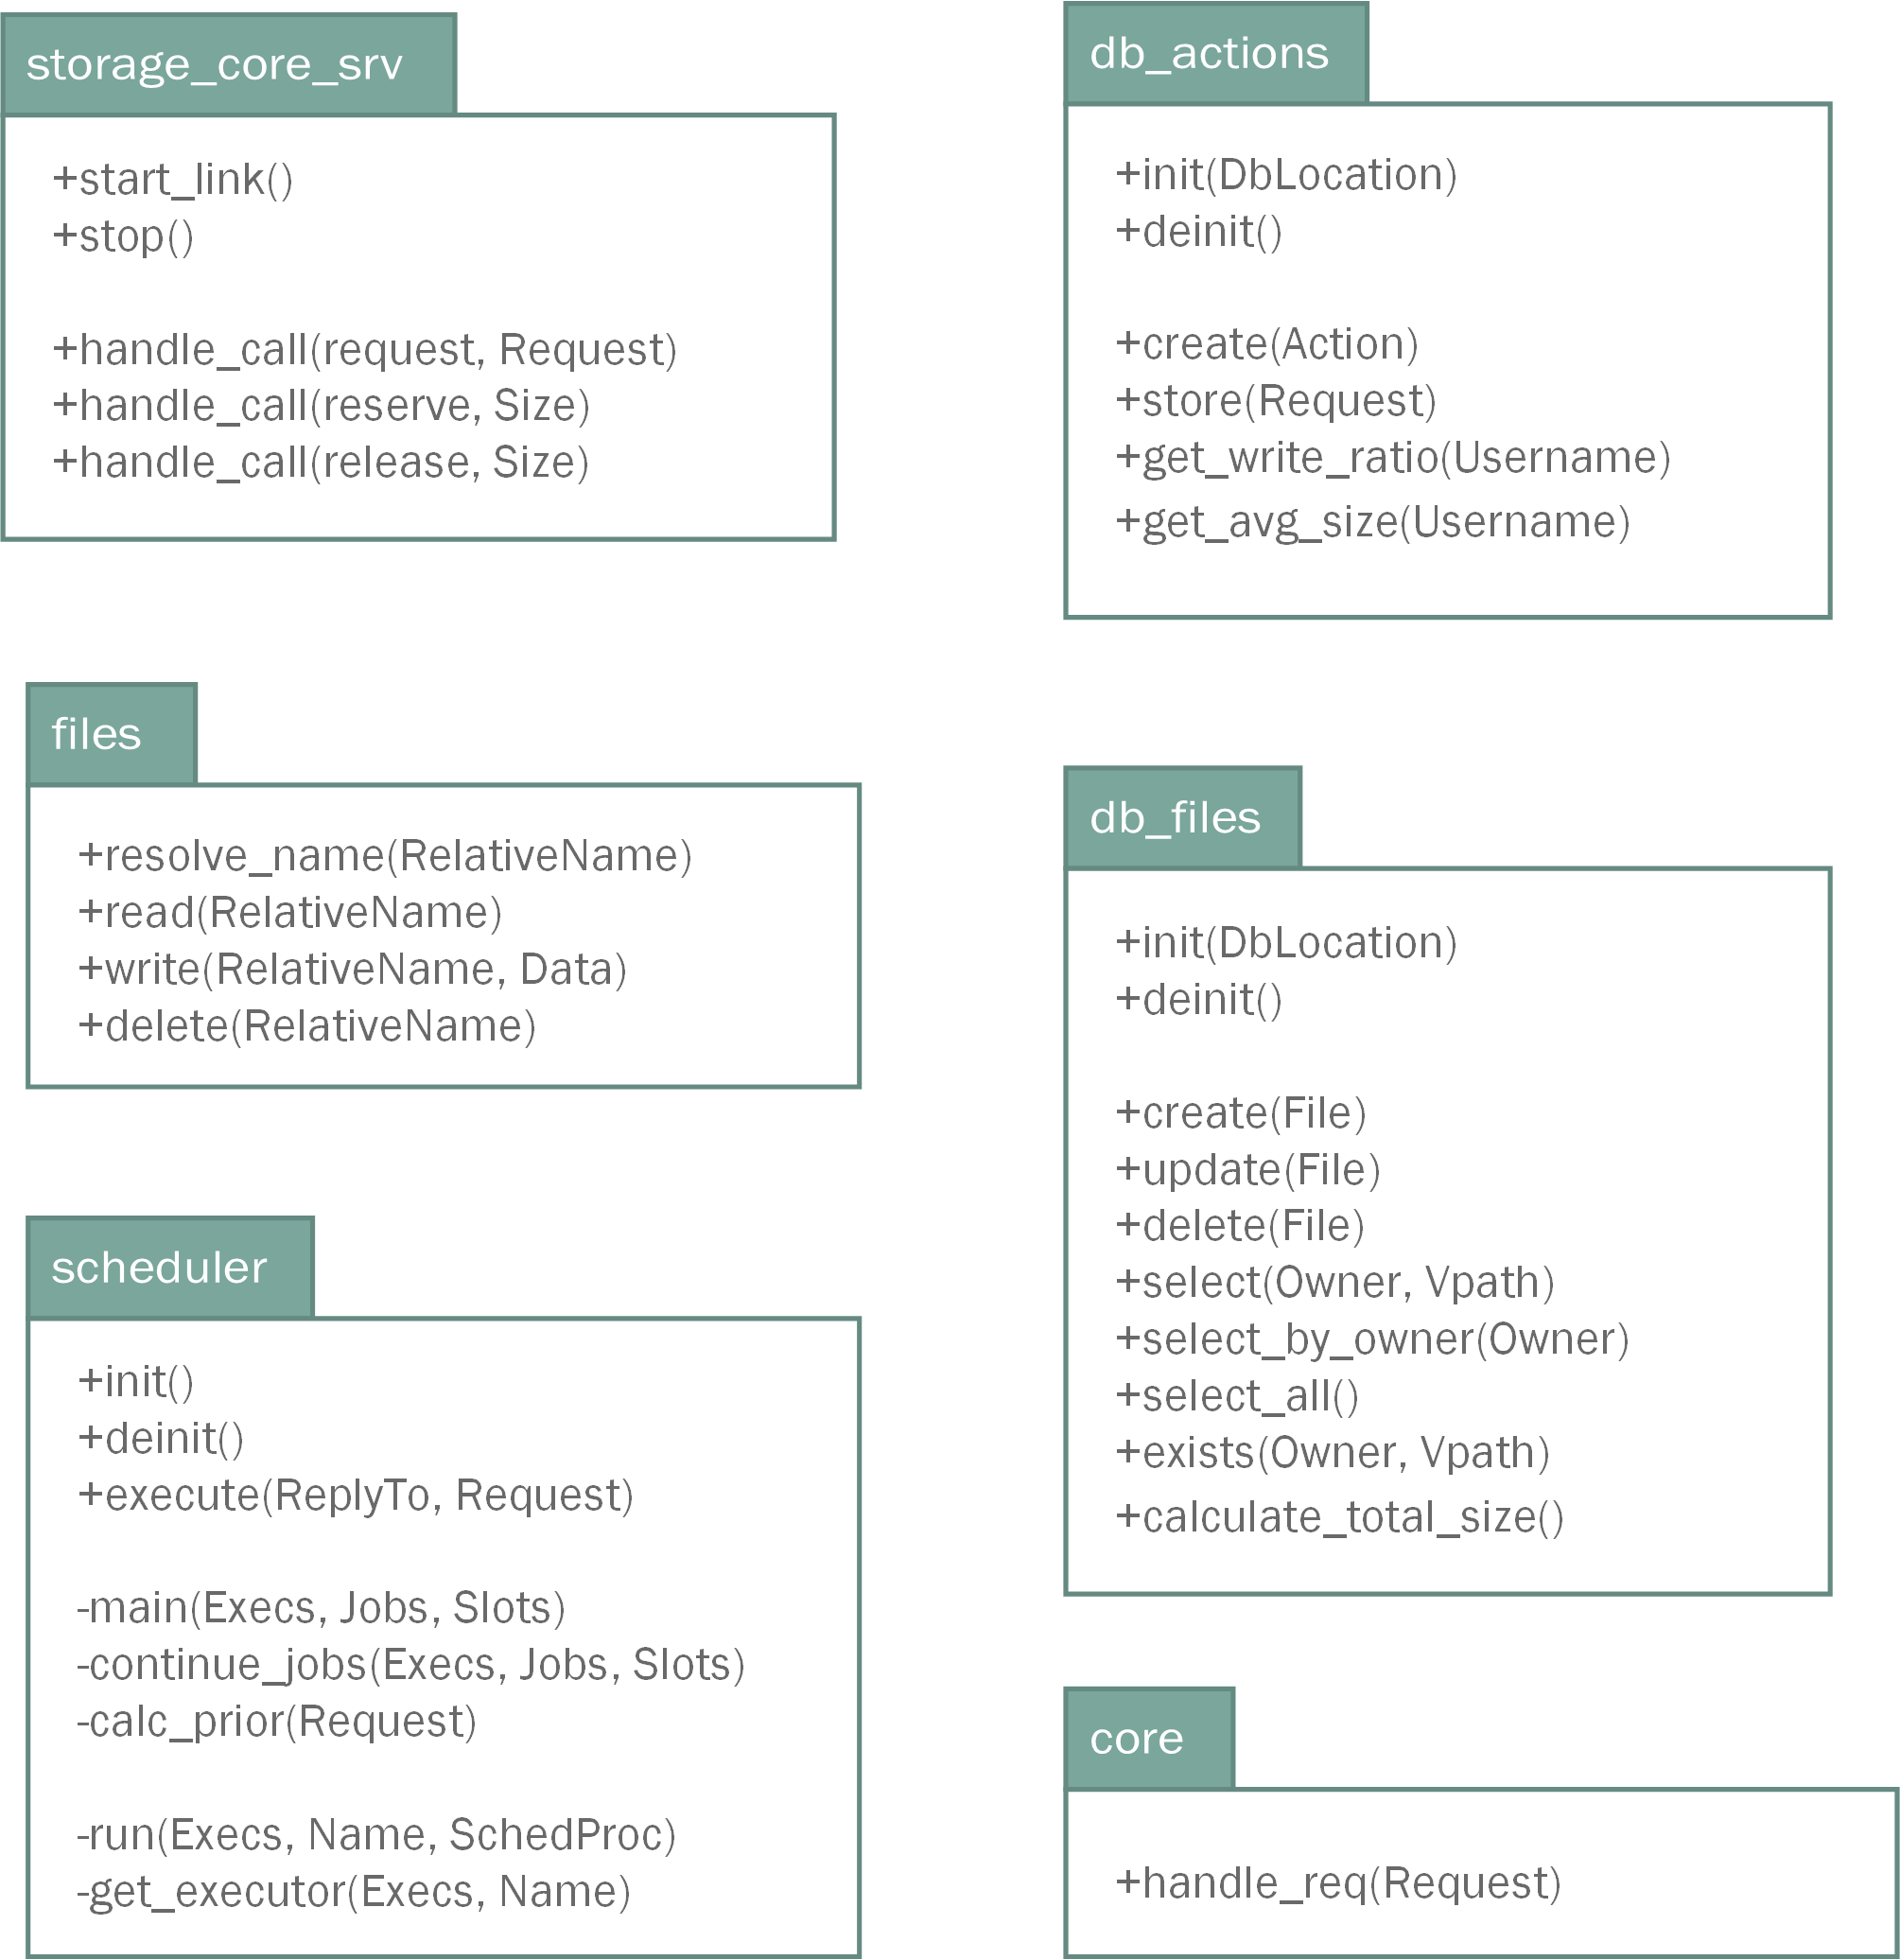
\includegraphics[width=0.9\textwidth]{core-module}
	\caption[Struktura modułu wykonawczego.]{Podmoduły składowe modułu core.}
	\label{fig:core-module}
\end{figure}

Każdy węzeł dysponuje określoną ilością miejsca na przechowywane pliki. Kiedy tworzone jest nowy plik, dostępne miejsce maleje. W punkcie 1.3.5 Moduł komunikacyjny przedstawiono zasady działania wywołań call(reserve, Size) i call(release, Size). Trzecia z funkcji gen\_servera, call(request, Request) odpowiedzialna jest za obsługę zapytania i przyjmuje w argumencie strukturę Request.
Zapytanie jest natychmiast przekazywane do modułu schedulera, który wyszukuje odpowiedni wątek wykonawczy i przekazuje mu zapytanie do obsługi. Wątek ten jest również odpowiedzialny za umieszczenie w bazie informacji o wykonanej akcji.
Ogólny diagram sekwencji przedstawia \autoref{fig:core-seq-1}. Rozważany przypadek to zapytanie read. Wszystkie inne wyglądają jednak tak samo. Scheduler został ukazany jako jeden, atomowy obiekt. Dalej opisany jest w szczegółach.

\begin{figure}[!htbp]
	\centering
	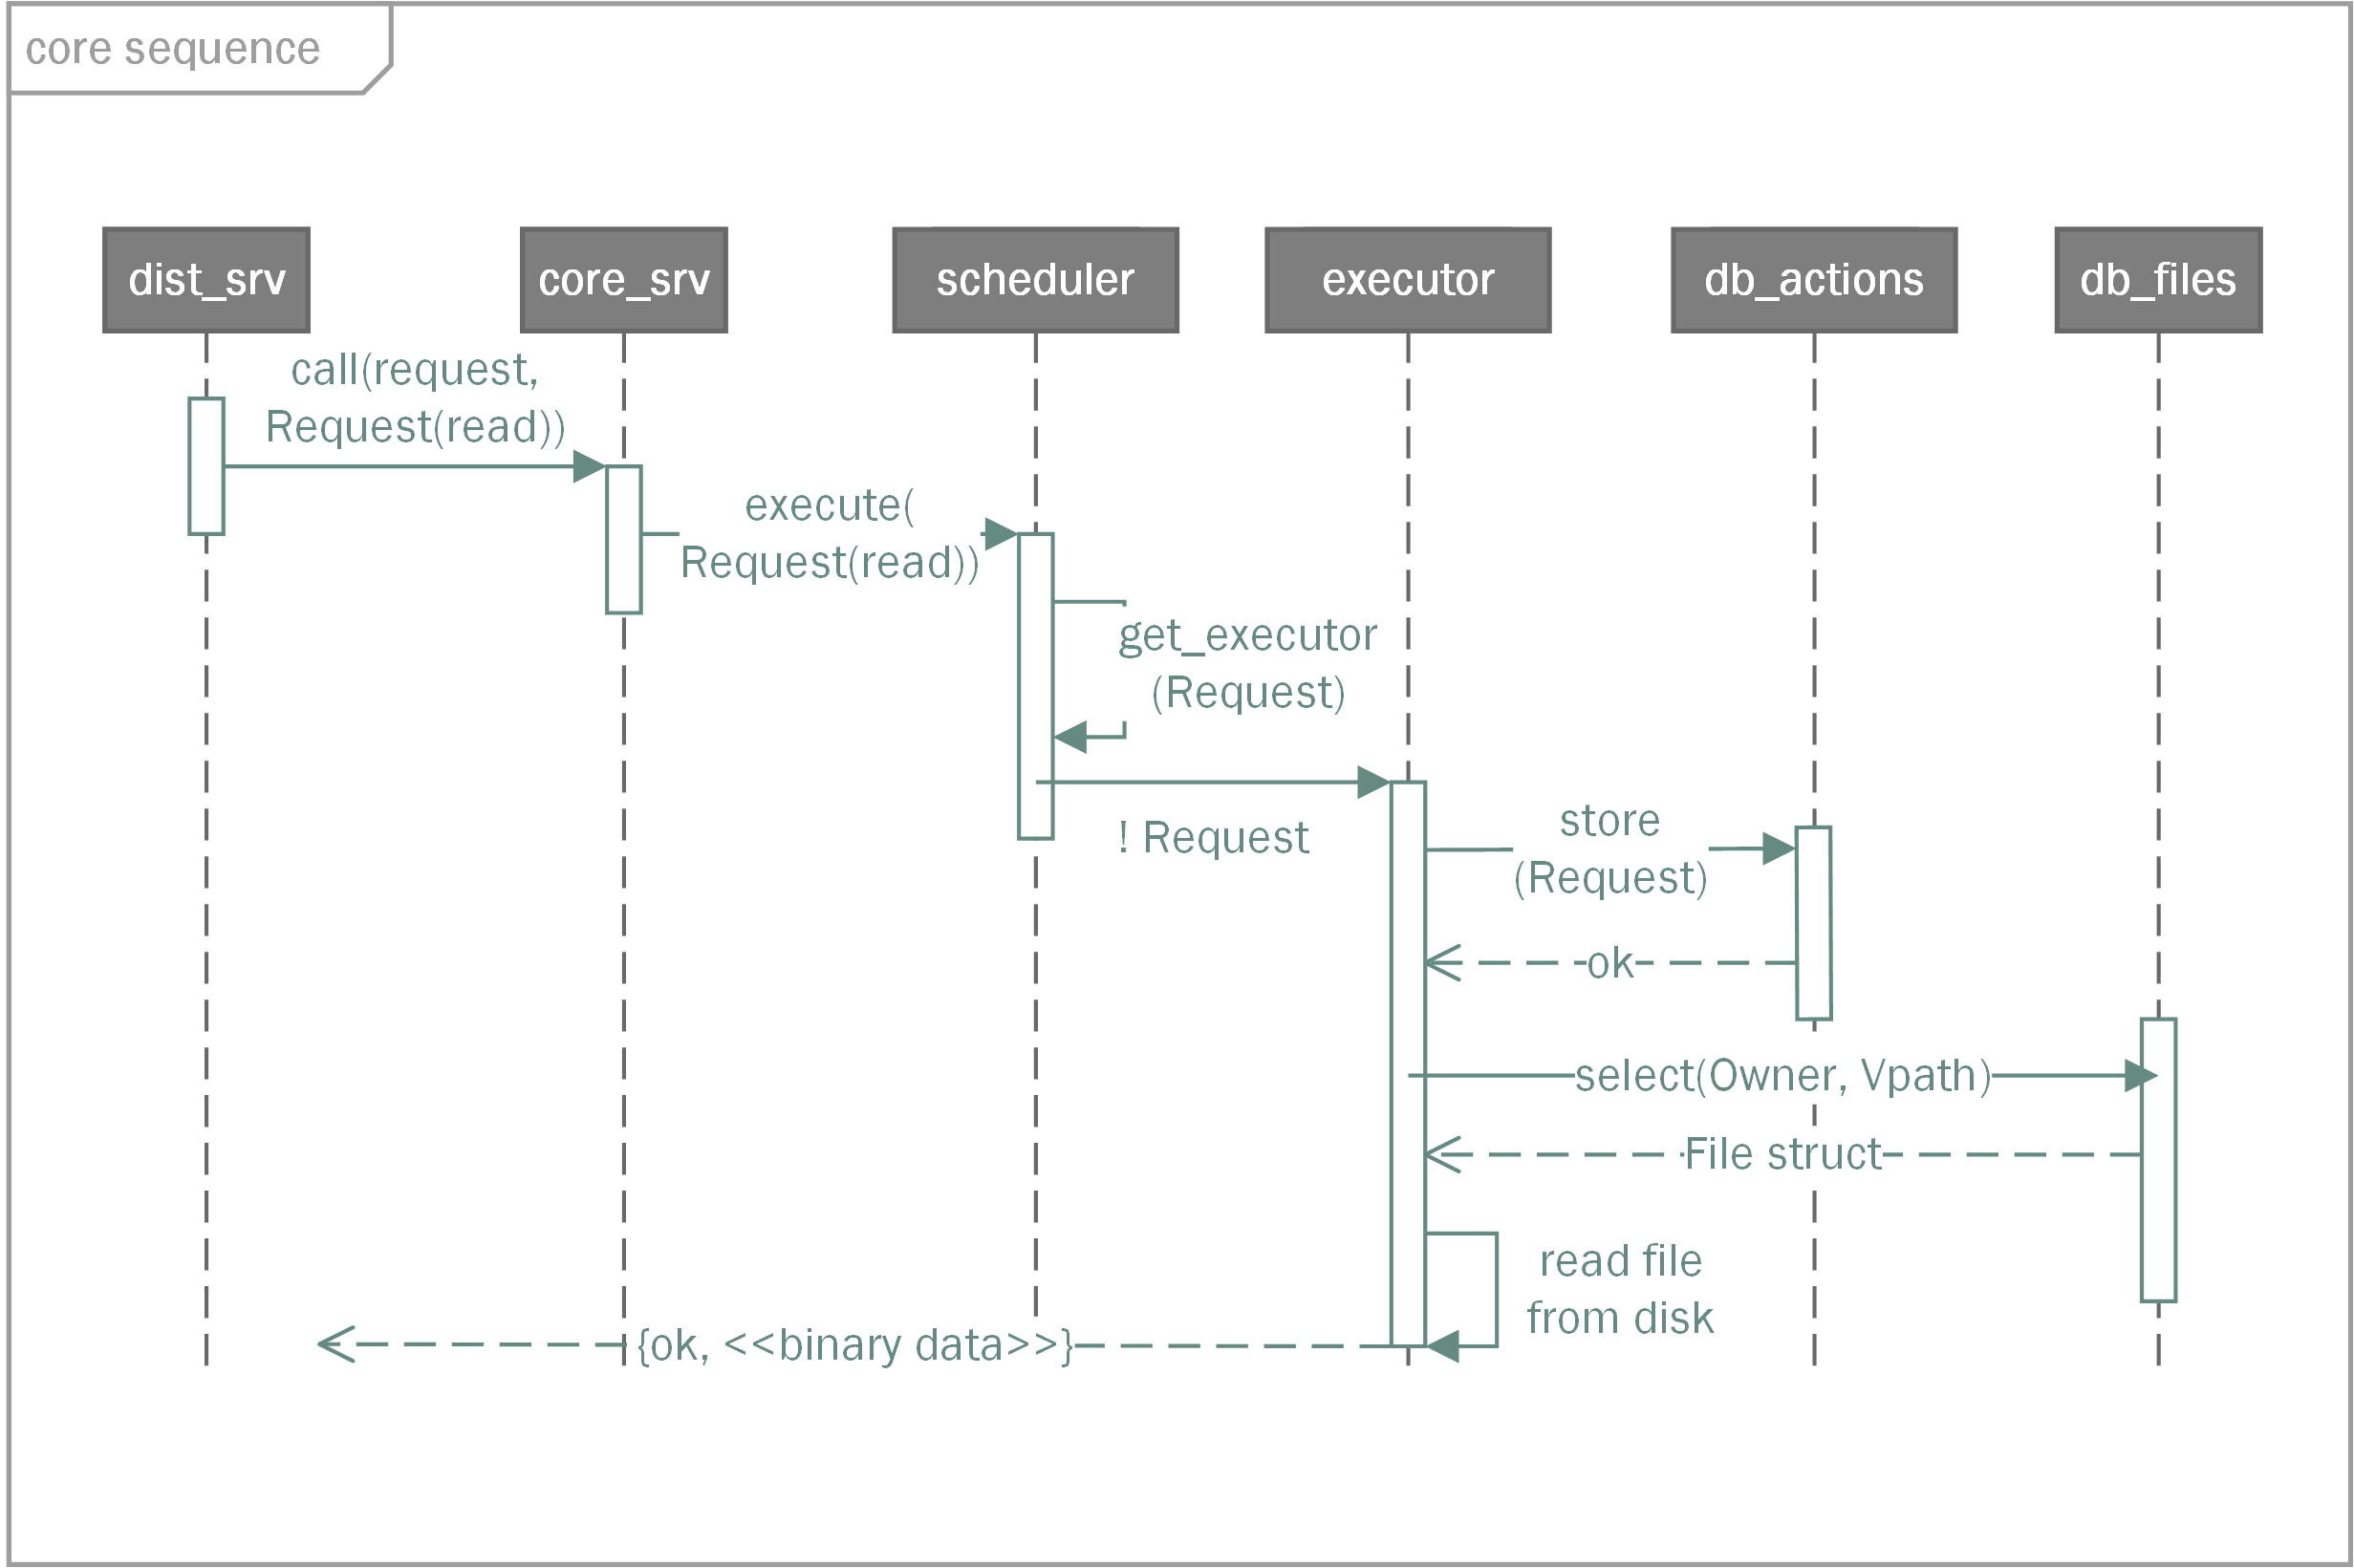
\includegraphics[width=0.9\textwidth]{core-seq-1}
	\caption{Obsługa żądania odczytu pliku w module wykonawczym.}
	\label{fig:core-seq-1}
\end{figure}

\paragraph{Scheduler} Scheduler jest modułem szeregującym zapytania trafiające do danego węzła. Zarządza on pulą wątków wykonawczych (executor), odpowiedzialnych za bezpośrednią obsługę zadań. Każdy plik (każda ścieżka) ma przydzielony jeden wątek wykonawczy. Zapytania dotyczące konkretnego pliku zawsze więc są obsługiwane przez jeden wątek. Wątek wykonawczy tworzony jest po próbie dostępu do określonego pliku i ulega zniszczeniu po określonym czasie bezczynności (domyślnie 180 sekund).

Po otrzymaniu zapytania o konkretny plik, scheduler znajduje skojarzony z nim wątek wykonawczy i umieszcza zadanie (strukturę Request) w kolejce wiadomości tego procesu (message queue języka Erlang).

Scheduler umieszcza wszystkie przychodzące akcje w kolejce priorytetowej. Zapisuje je w postaci krotek \{Priority, Executor\}, gdzie Priority to priorytet obliczony dla danego zapytania natomiast Executor to identyfikator wątku wykonawczego gdzie trafiło to zapytanie.

Przed rozpoczęciem przetwarzania kolejnego zadania, wątek wykonawczy czeka na pozwolenie od schedulera. Po każdym zakończonym zadaniu informuje scheduler o zakończeniu jego obsługi.

Scheduler uruchamia N (domyślnie 4) pierwszych wątków wykonawczych z kolejki priorytetowej. Jeżeli jakiś wątek skończy przetwarzać jakieś zapytanie, scheduler wybiera z kolejki w jego miejsce wątek o najwyższym priorytecie.

\begin{figure}[!htbp]
	\centering
	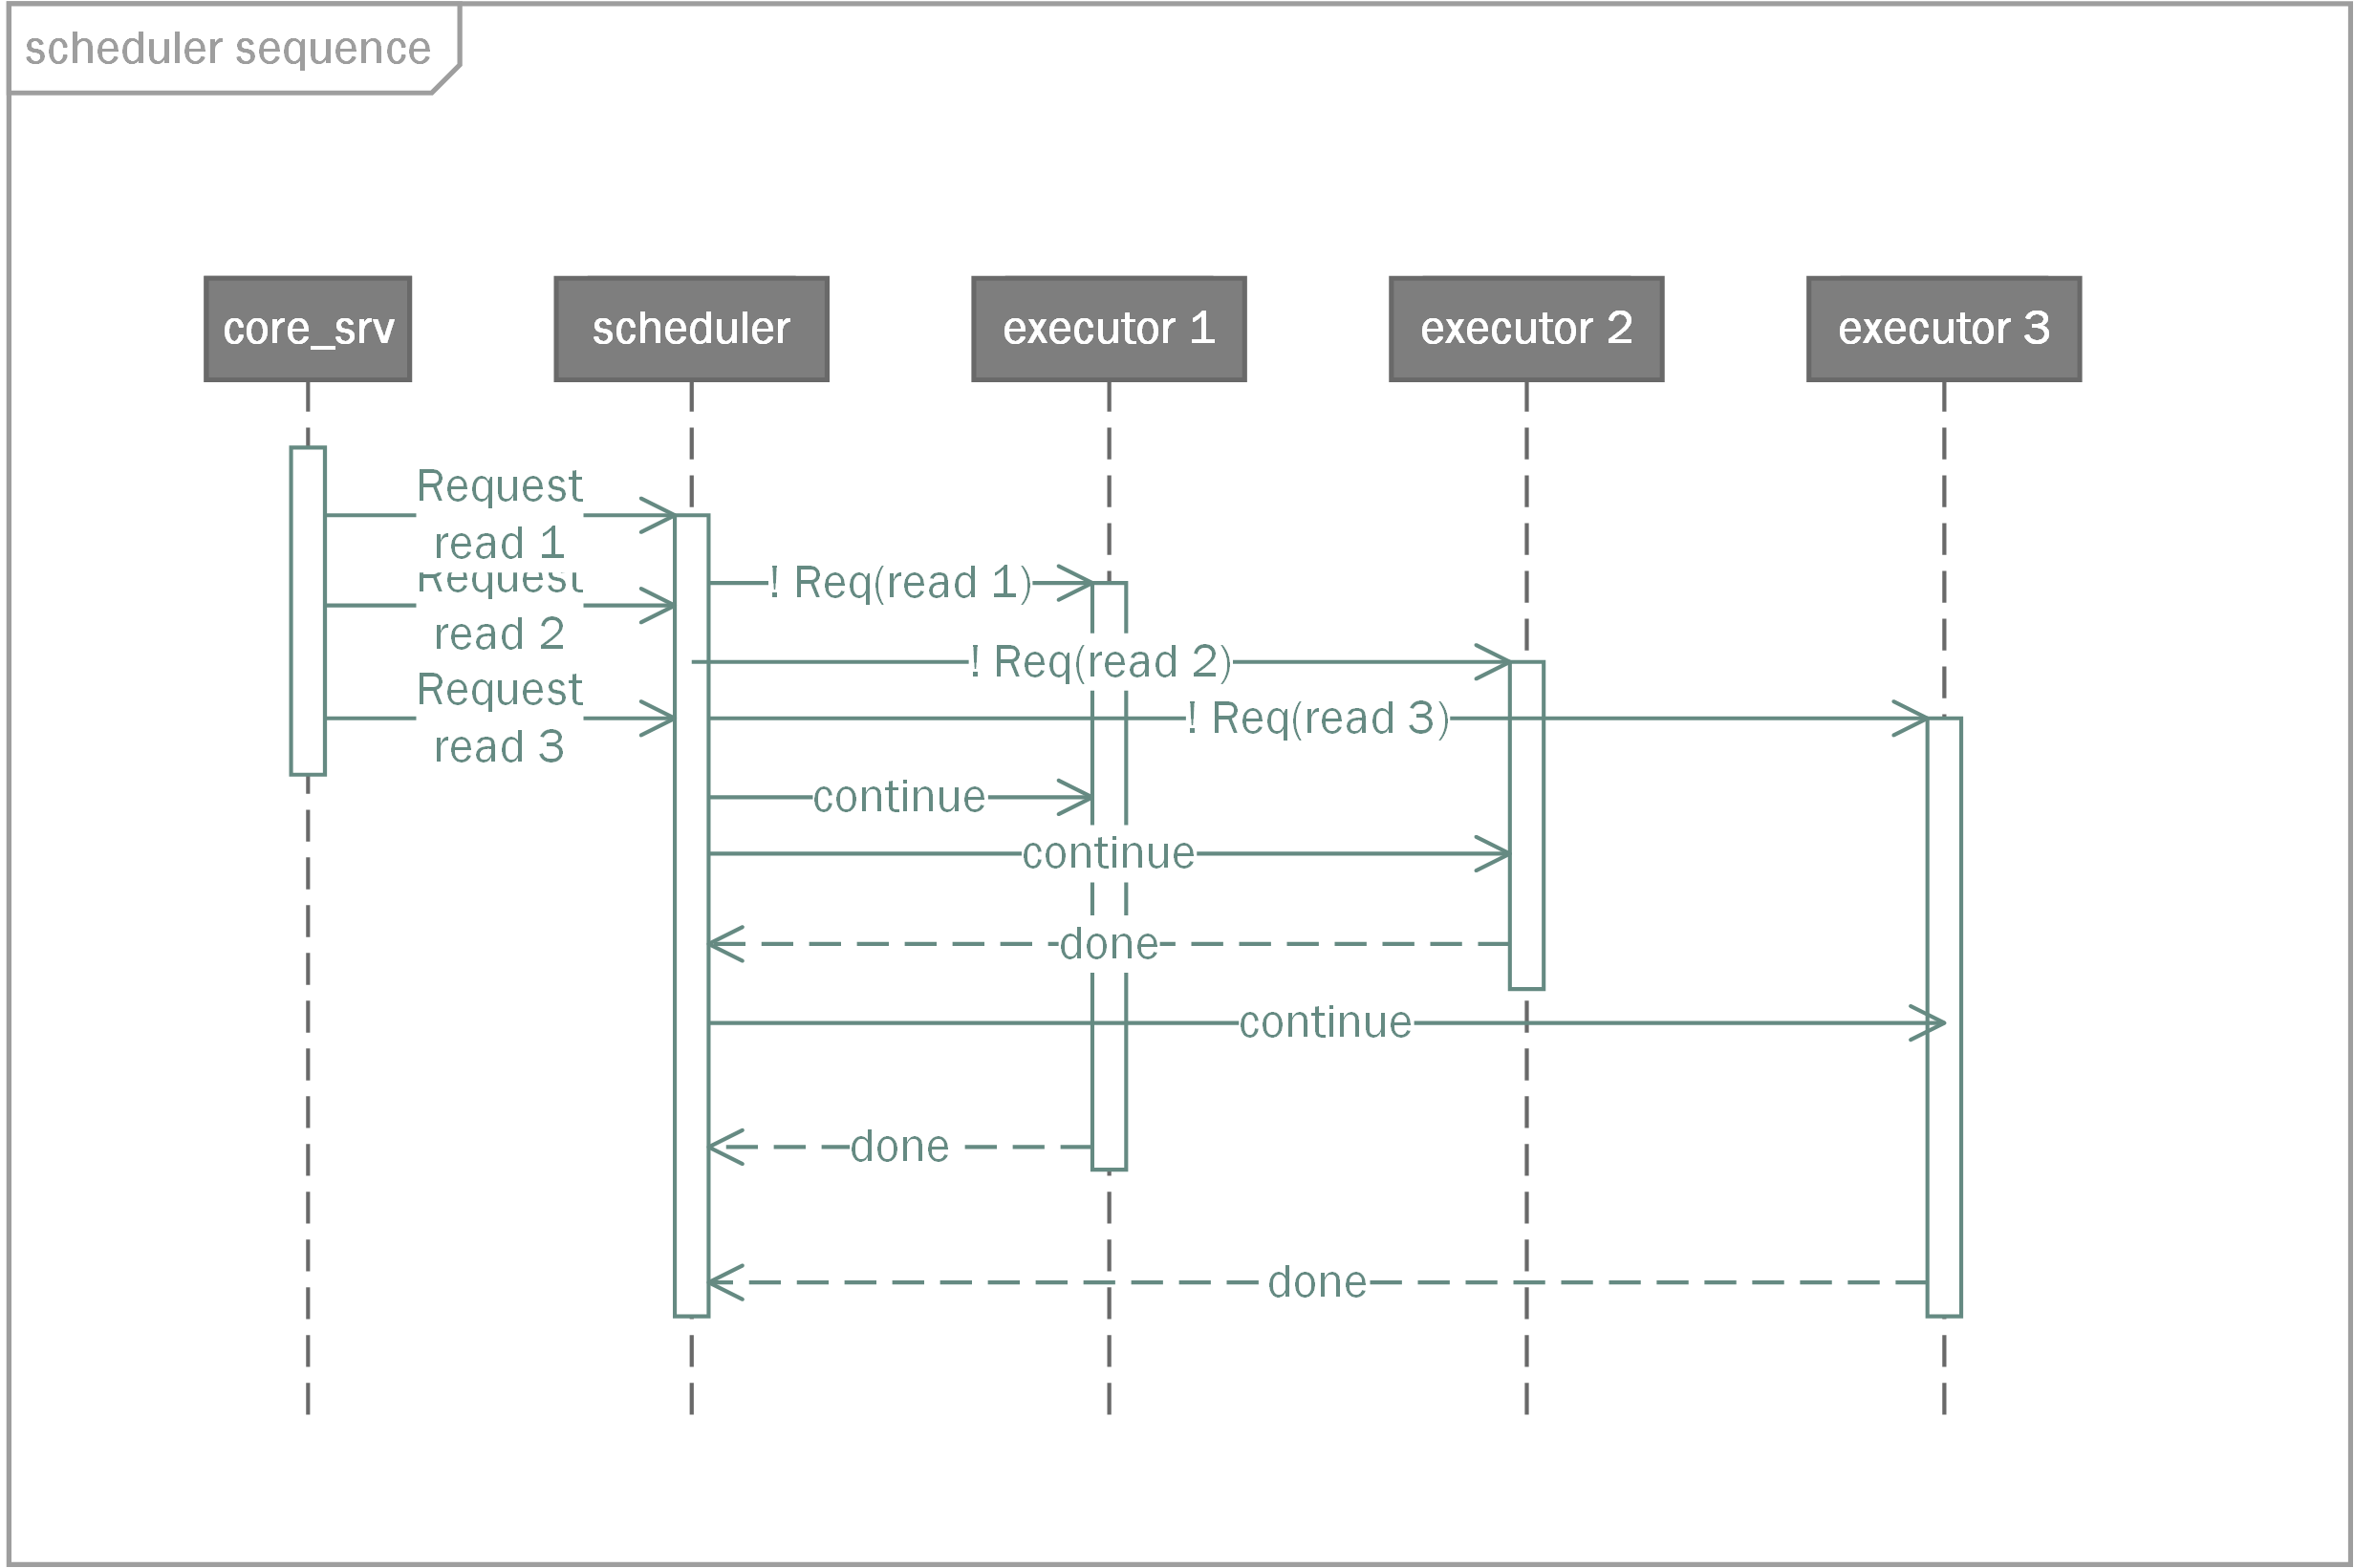
\includegraphics[width=0.9\textwidth]{core-seq-2}
	\caption[Sekwencja uruchamiania wątków wykonawczych.]{Sekwencja uruchamiania wątków wykonawczych (maksymalnie dwa jednoczesne wątki). Pojawiają się trzy zapytania o trzy różne pliki. Każde z nich trafi zatem do innego wątku wykonawczego. Zadania są kolejkowane w wątkach zgodnie z kolejnością przybycia (kolejność w obrębie jednego wątku wykonawczego musi zostać zachowana). Wątki nie rozpoczynają pracy od razu – scheduler wysyła do każdego z nich komunikat continue. Dwa wątki zostały uruchomione jednocześnie. Trzeci czekał na zakończenie pracy przez jeden z nich.}
	\label{fig:core-seq-2}
\end{figure}

\subsubsection{Baza danych}
System korzysta z bazy danych SQLite3. W celu komunikacji z bazą danych z poziomu Erlanga wybrano erlang-sqlite3 (\url{https://github.com/alexeyr/erlang-sqlite3}). Persystowane są trzy rodzaje struktur: User, File oraz Action. Opisuje je rozdział 1.2 Struktury. Dla każdej z nich zdefiniowany jest odpowiedni moduł DAO: db\_users, db\_files oraz db\_actions. Wszystkie zostały przedstawione w poprzednich rozdziałach przy omawianiu modułów nadrzędnych.

Moduły DAO znajdują się w plikach:
\begin{itemize}
	\item storage/src/core/db\_files.erl
	\item storage/src/auth/db\_users.erl
	\item storage/src/core/db\_actions.erl
\end{itemize}

W przypadku chęci zmiany bazy danych, zmian wystarczy dokonać tylko w tych plikach (oraz dostarczyć odpowiedni sterownik). Jeden z prototypów działał z wykorzystaniem bazy MySQL.

\begin{figure}[!htbp]
	\centering
	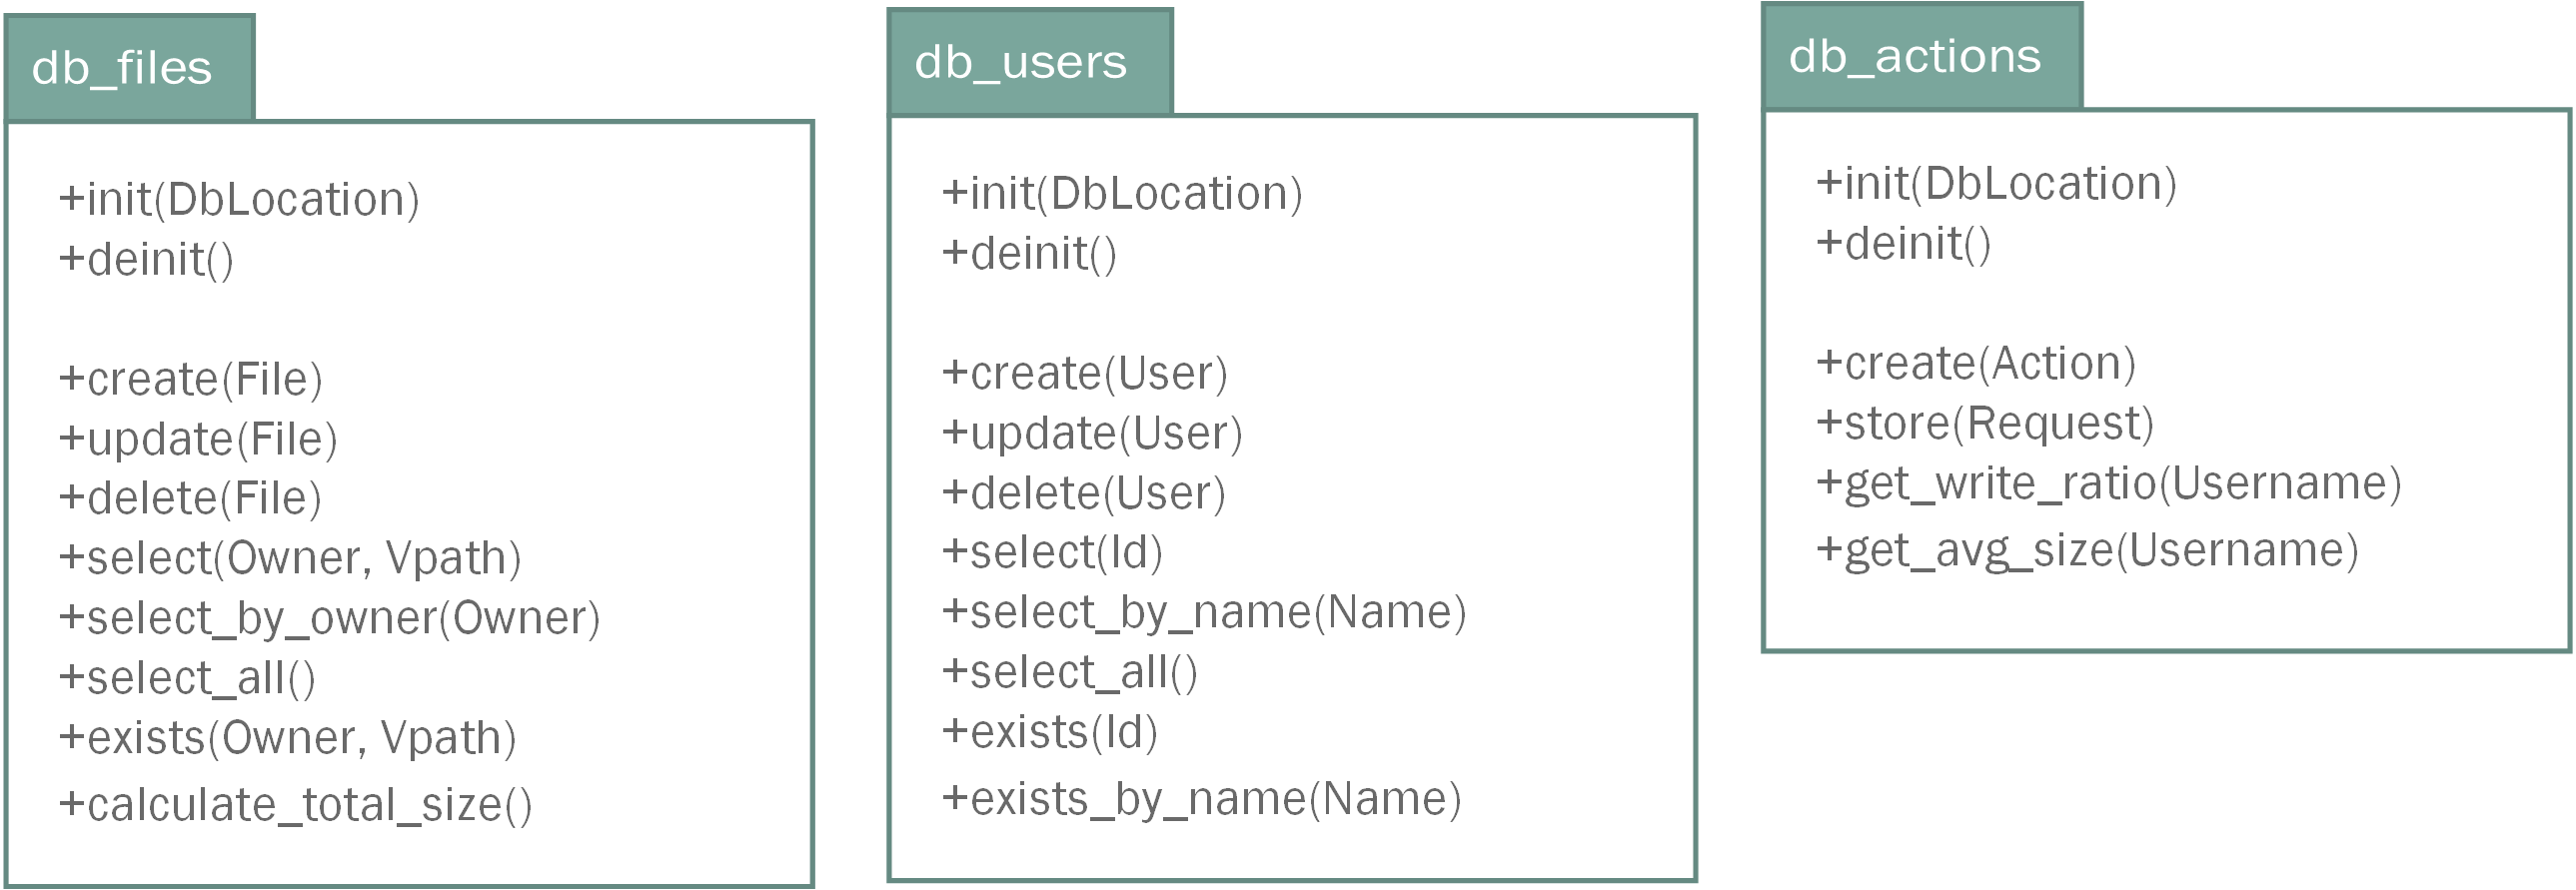
\includegraphics[width=0.9\textwidth]{db-modules}
	\caption[Struktura modułów DAO.]{Moduły DAO pozwalają zapisywać obiekty w bazie danych i wyszukiwać je na podstawie identyfikatora.}
	\label{fig:db-modules}
\end{figure}

\autoref{fig:db-erd} przedstawia diagram ERD bazy danych. Struktura tabel jest bardzo prosta jednak pozwala zrealizować wszystkie wymagania projektu.

Baza może pracować w standardowo, zapisując rekordy na dysku oraz w konfiguracji in-memory. Druga opcja przydatna może być w testach wydajnościowych. W celu jej aktywacji należy skompilować projekt z odpowiednią flagą. Więcej na temat kompilacji mówi rozdział 3.3 Kompilacja.

\begin{figure}[!htbp]
	\centering
	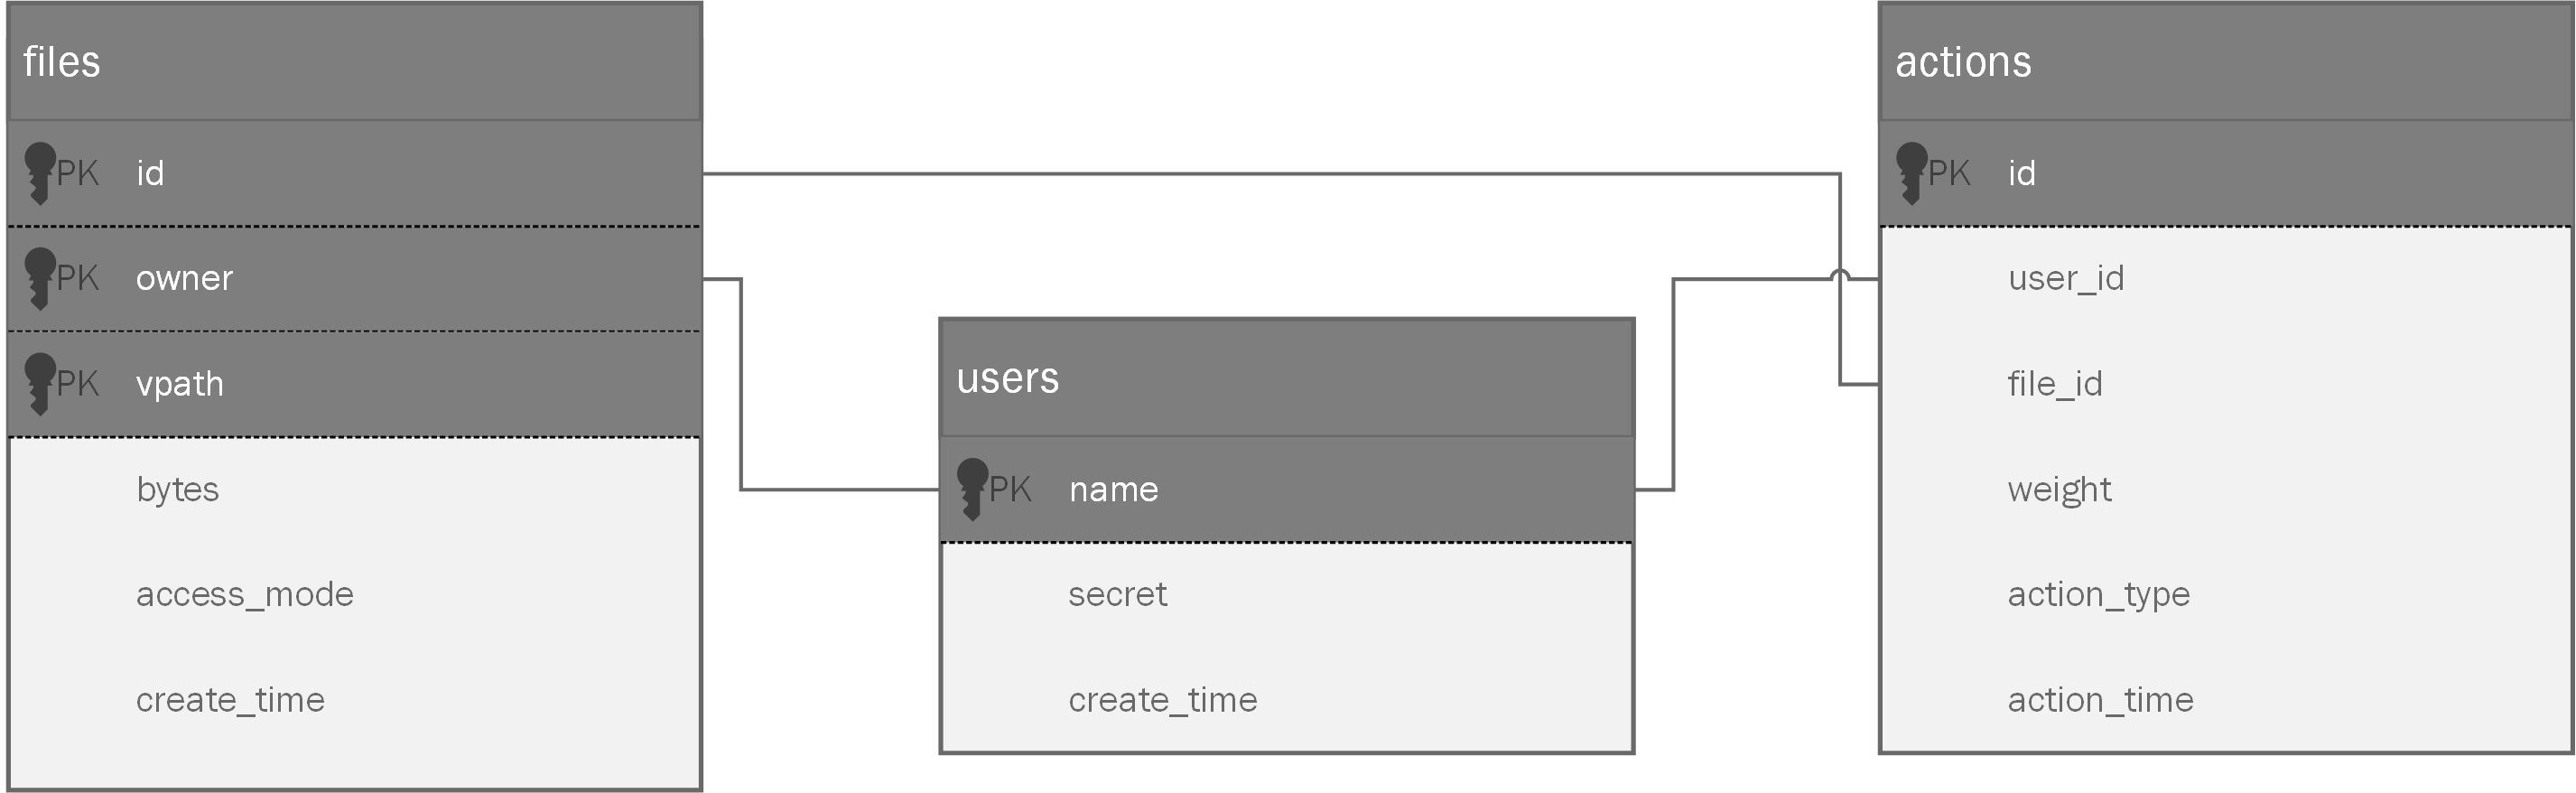
\includegraphics[width=0.9\textwidth]{db-erd}
	\caption{Baza danych - diagram ERD}
	\label{fig:db-erd}
\end{figure}
\subsubsection{Generator UUID}
Struktura:
\begin{itemize}
	\item storage/src/shared/storage\_uuid\_srv.erl – gen\_server
\end{itemize}

Jest to wielowątkowy moduł służący do generowania unikalnych, 128-bitowych identyfikatorów. Identyfikatory te są wykorzystywane jako nazwy fizycznych plików przechowywanych w systemie dyskowym. Właściwymi identyfikatorami plików i użytkowników w systemie pozostają jednak zwykłe napisy, w postaci czytelnej dla człowieka.

Strukturę modułu przedstawia diagram z \autoref{fig:uuid-module}. Jedyna publiczna funkcja służy do generowania identyfikatora. Dla każdego wywołania uruchamiany jest osobny wątek. Identyfikator zwracany jest w postaci typu binary().

\begin{figure}[!htbp]
	\centering
	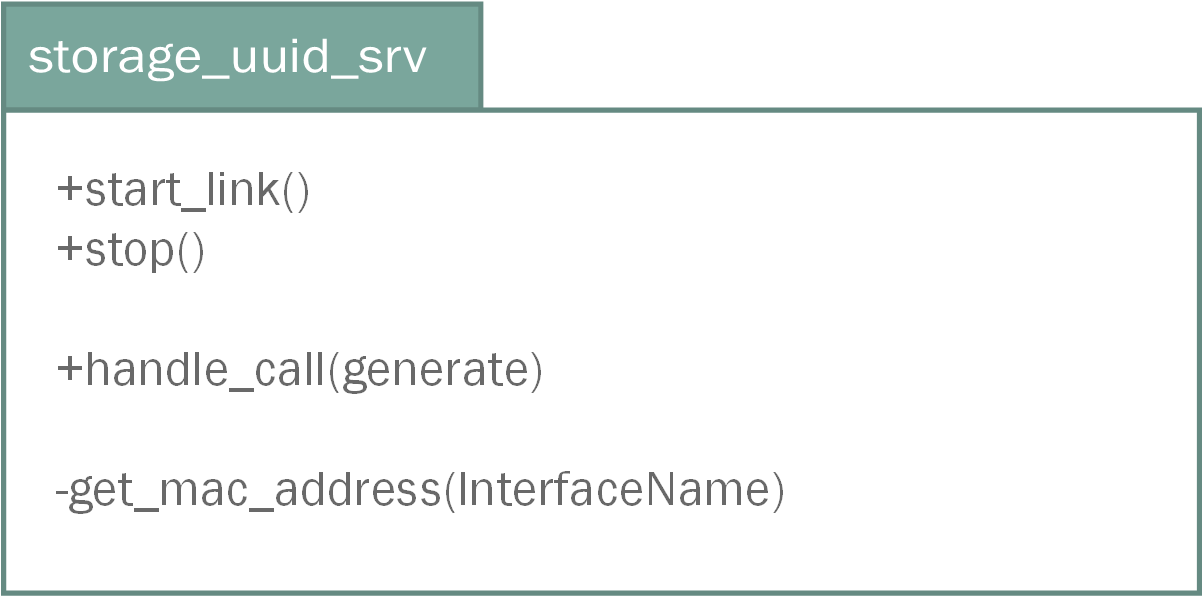
\includegraphics[width=0.7\textwidth]{uuid-module}
	\caption{Interfejs modułu storage\_uuid\_srv.}
	\label{fig:uuid-module}
\end{figure}

Identyfikator składa się z trzech części – grup bitów, z których każda ma odpowiednią interpretację:

\centerline{\texttt{<< 48bit timestamp, 48bit adres MAC, 32bit losowa wartość >>}}

48-bitowy znacznik czasowy przechowuje czas wygenerowania identyfikatora (UNIX time) z dokładnością do milisekund. Adres MAC pobierany jest z określonego w pliku konfiguracyjnym interfejsu sieciowego (domyślnie eth0). Zastosowanie składnika w postaci MAC gwarantuje, że generowane identyfikatory są unikalne w obrębie całego systemu. Ostatni składnik identyfikatora to 32 losowe bity. Daje to 4 294 967 296 możliwych do wygenerowania unikalnych identyfikatorów w ciągu milisekundy.
\subsubsection{Logger}
Struktura:
\begin{itemize}
	\item storage/src/shared/log.erl – moduł
\end{itemize}

Moduł loggera. Wypisuje komunikaty na standardowe wyjście. Węzeł zbudowany w trybie release nie posiada uruchomionej konsoli. Wtedy logi trafiają w domyślne miejsce: log/erlang.log.1

Interfejs loggera przedstawia \autoref{fig:log-module}. Dostępne są trzy funkcje logujące informacje: log:info, log:warn oraz log:error. Pozwalają logować informacje różnych typów. O tym, czy dana funkcja wypisze komunikat na ekran decyduje poziom logowania ustawiony w konfiguracji aplikacji. Szczegóły przedstawia rozdział 3.5 Pliki konfiguracyjne. Możliwe poziomy logowania:
\begin{itemize}
	\item info: wszystkie funkcje wypisują komunkaty. Z użyciem tej funkcji wypisywane są informacje o zdarzeniach aktualnie zachodzących w systemie.
	\item warn: wywołania log:info są ignorowane. . Przy użyciu tej funkcji wypisywane są przykładowo informacje o niepoprawnej sumie kontrolnej
	\item error: wywołania log:info oraz log:warn są ignorowane. Zarezerwowana jest dla krytycznych błędów.
	\item none: wszystkie funkcje są ignorowane, nic nie jest wypisywane
\end{itemize}

Interfejs tych trzech funkcji jest identyczny. Każa występuje w dwóch wersjach:
\begin{itemize}
	\item log:xxxx(Message) – wypisuje wiadomość (typu string())
	\item log:xxxx(Format, [Args]) – wypisuje sformatowany napis (string()) z wstawionymi argumentami. Obowiązuje standardowe formatowanie jak we wbudowanym module io.
\end{itemize}

\begin{figure}[!htbp]
	\centering
	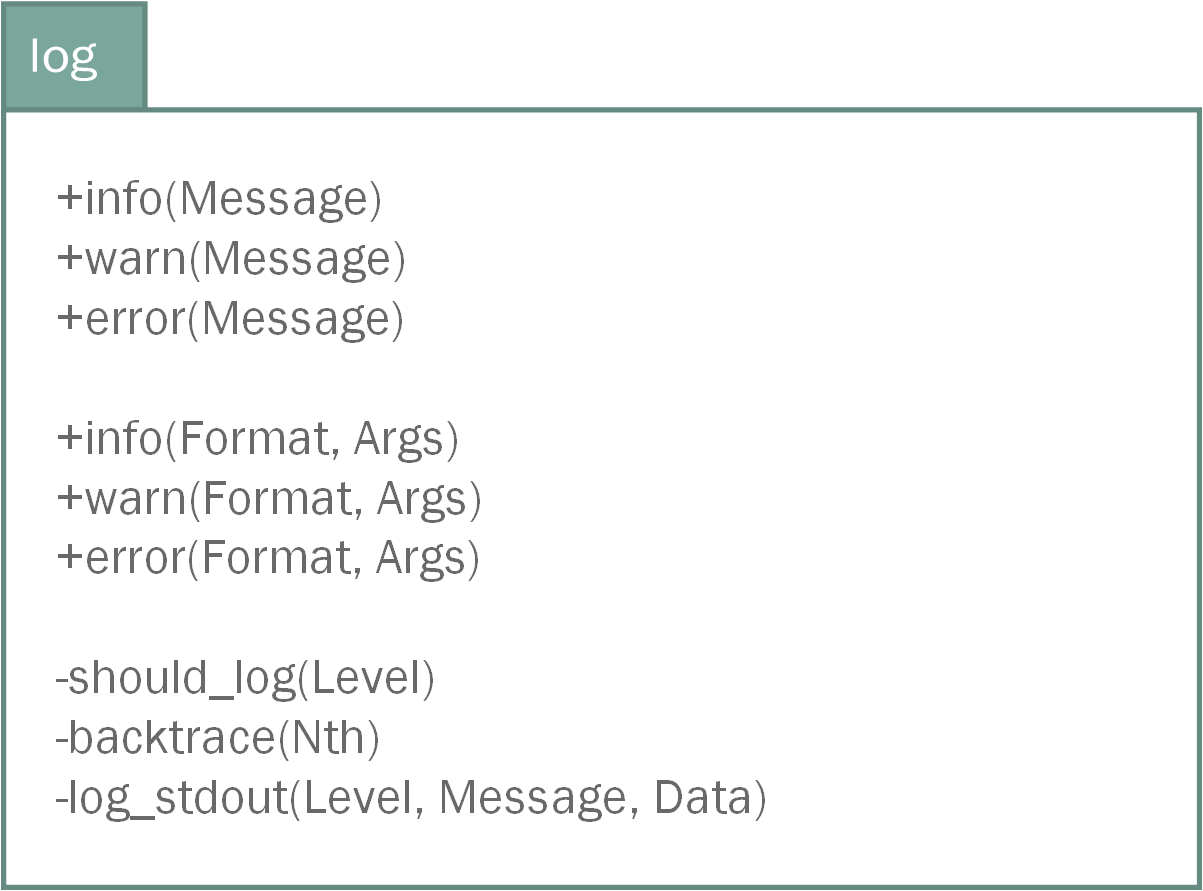
\includegraphics[width=0.7\textwidth]{log-module}
	\caption{Struktura modułu loggera.}
	\label{fig:log-module}
\end{figure}

Wypisany komunikat ma strukturę:

\centerline{\texttt{[level] HH:MM:SS (module:function/arity): message}}

Przykładowo:
\begin{lstlisting}
[info] 18:51:33 (storage_dist_srv:handle_cast/2):
			'ds3@michal-pc' has joined the cluster!
\end{lstlisting}

Określenie lokalizacji (funkcji, z której nastąpiło logowanie) odbywa się automatycznie, poprzez symulowane rzucenie wyjątku, złapanie go, a następnie zbadanie stosu wywołań. Może do negatywnie wpływać na wydajność. Logowanie można więc całkowicie zablokować odpowiednią opcją kompilacji.

\subsubsection{Biblioteka kliencka}
Struktura:
\begin{itemize}
	\item storage/src/client/storage.erl – moduł
\end{itemize}

Biblioteka kliencka jest zwykłym modułem języka Erlang. Publiczny interfejs oferuje sześć funkcji, odpowiadających oferowanej przez system funkcjonalności tworzenia (storage:create), czytania (storage:read), aktualizowania (storage:update), usuwania (storage:delete), listowania (storage:list) oraz wyszukiwania plików (storage:find). Moduł przedstawiony jest na \autoref{fig:client-module}.

\begin{figure}[!htbp]
	\centering
	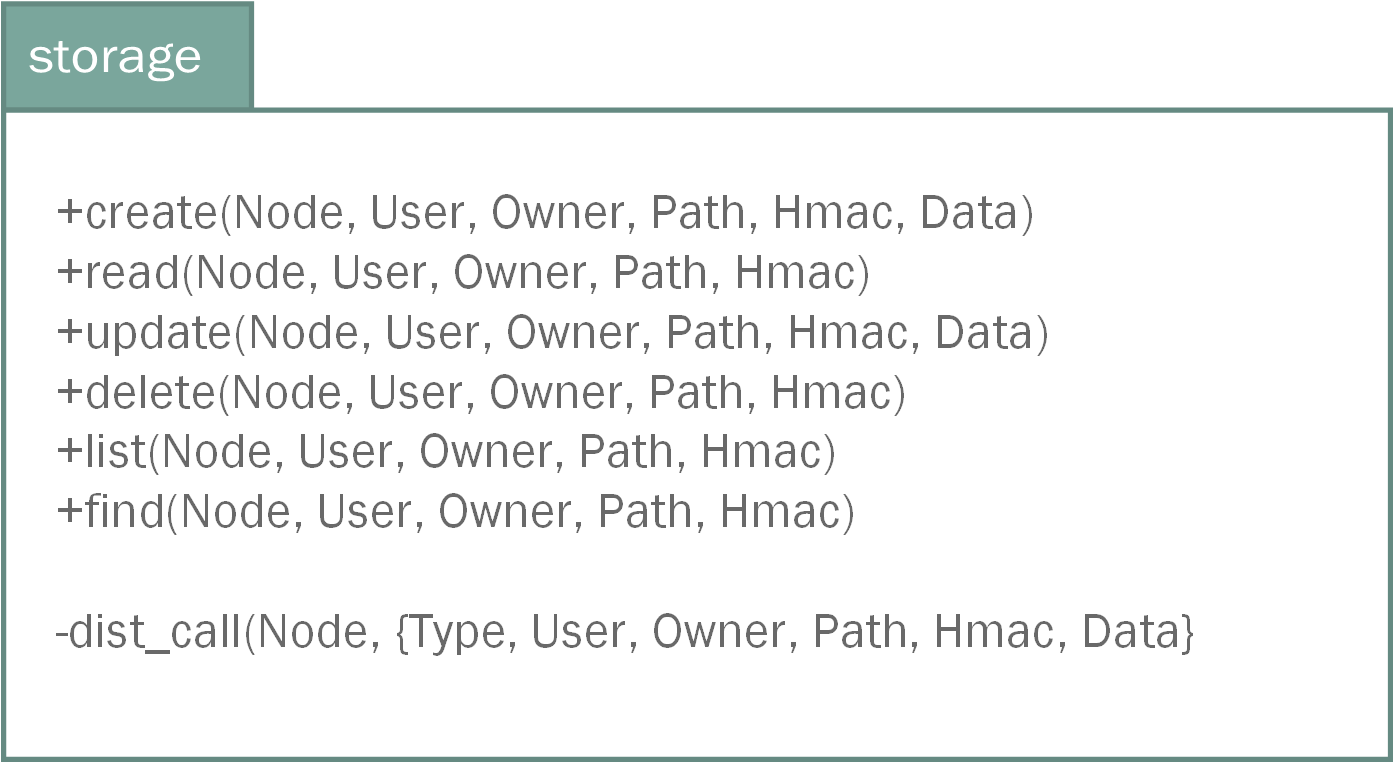
\includegraphics[width=0.7\textwidth]{client-module}
	\caption{Moduł biblioteki klienckiej.}
	\label{fig:client-module}
\end{figure}

Wszystkie funkcje mają identyczną sygnaturę. Dodatkowo, storage:create oraz storage:update w ostatnim argumencie przyjmują dodatkowy argument – zapisywany plik w postaci danych binarnych. Kolejne argumenty to:
\begin{itemize}
	\item Node – adres węzła docelowego (gateway node). Zapytanie trafi do modułu storage\_dist\_srv na wskazanym węźle.
	\item User – identyfikator (nazwa) użytkownika wykonującego zapytanie.
	\item Owner – identyfikator właściciela pliku, do którego odnosi się zapytanie.
	\item Path – ścieżka do pliku (zgodna z konwencją adresowania w systemie). Musi być unikatowa.
	\item Hmac – suma kontrolna HMAC-SHA1, obliczona z całego, skonkatenowanego ciała zapytania, zaszyfrowana sumą SHA1 obliczoną z hasła użytkownika (kluczem prywatnym)
	\item Data – dane binarne
\end{itemize}

Sposób działania wszystkich funkcji jest identyczny. Konstruują odpowiednią strukturę Request, wysyłają ją do wskazanego węzła (proces storage\_dist\_srv) a następnie oczekują na odpowiedź.

Odpowiedzi mają postać:
\begin{itemize}
	\item {ok, SuccessResponse}
	\item {error, Reason}
\end{itemize}

W przypadku pozytywnej odpowiedzi, SuccessResponse do binarna zawartość odczytanego pliku w przypadku zapytania read, lista adresów wszystkich plików w przypadku zapytania list czy też adres węzła przechowującego dany plik w przypadku zapytania find.

Reason to zawsze atom, opisujący przyczynę błędu, przykładowo not\_found.


\subsection{GUI}
TODO